\lstinputlisting[language=bash,basicstyle=\small]{python_codes/fieldstone_77/keywords}

\begin{center}
Code at \url{https://github.com/cedrict/fieldstone/tree/master/python_codes/fieldstone_77}
\end{center}

\par\noindent\rule{\textwidth}{0.4pt}

%%%%%%%%%%%%%%%%%%%%%%%%%%%%%%%%%%%%%%%%%%%%%%%%%%%%%%%%%%%%%%%%%%%%%%%%%%%%%%%%%%%%%%%%%%%%

I have implemented the two variants of the Rannacher-Turek element presented
in Section~\ref{ss:RTq1p0}, the mid-value (MV) and the mid-point (MP).
After communicating with Prof. Turek, I also implemented the Laplace 
formulation of the Stokes equation, i.e. we assume $\eta$ to be constant 
and therefore for an incompressible flow the momentum conservation 
equation becomes 
\[
-\vec\nabla p + \eta \Delta \vec\upnu + \rho \vec{g} = \vec{0}
\]
This yields a different form of the viscous block of the Stokes system
as explained in Section~\ref{ss:isovisc}.
I use an isoparametric mapping, but I have tried a $Q_1$ mapping and given that 
all elements are square it does not change anything. 

Following a discussion with W. Bangerth, I have also implemented the DSSY element 
(see Section~\ref{ss:dssy_2D}) which 'lives' on the same four nodes placed at 
the mid-edges. DSSY(1) corresponds to the basis functions based on $\theta_1$ 
while DSSY(2) corresponds to the basis functions based on $\theta_2$ \cite{doss99}

In what follows formulation 1 stands for the regular form of the 
Stokes equation, while formulation 2 stands for the Laplace one.

I have implemented four benchmarks based on manufactured solutions:
\begin{itemize}
\item Donea-Huerta, see Section~\ref{mms1}

\begin{center}
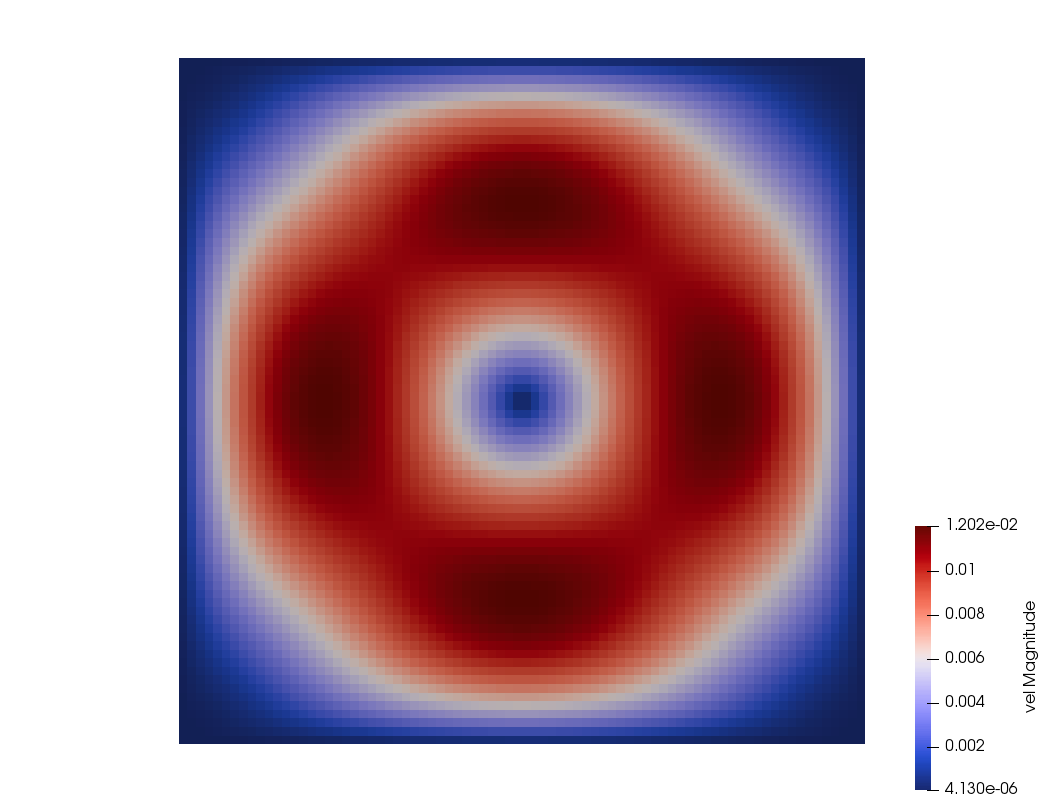
\includegraphics[width=7cm]{python_codes/fieldstone_77/results/dh/vel}
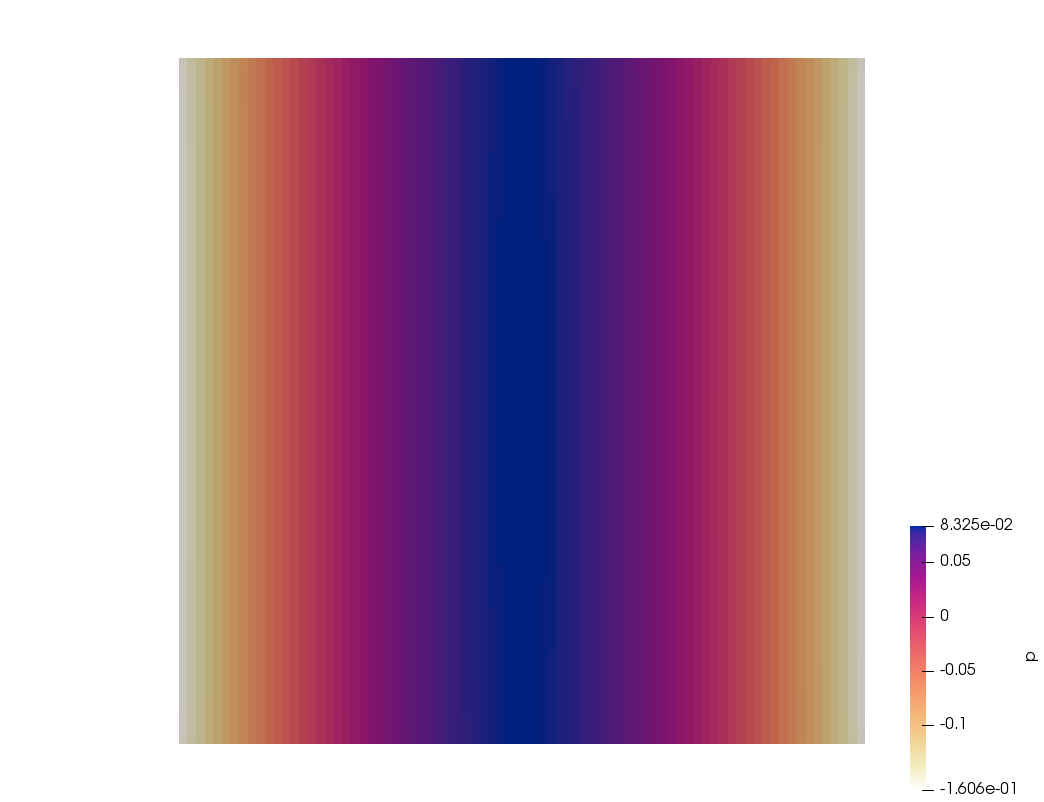
\includegraphics[width=7cm]{python_codes/fieldstone_77/results/dh/press}\\
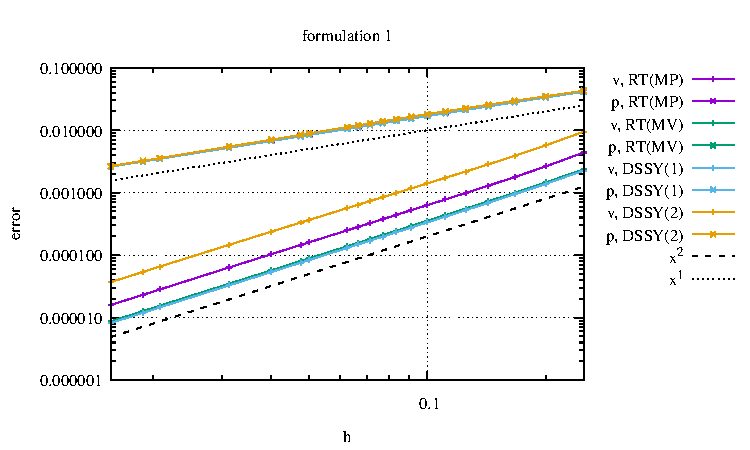
\includegraphics[width=8cm]{python_codes/fieldstone_77/results/dh/errors_form1}
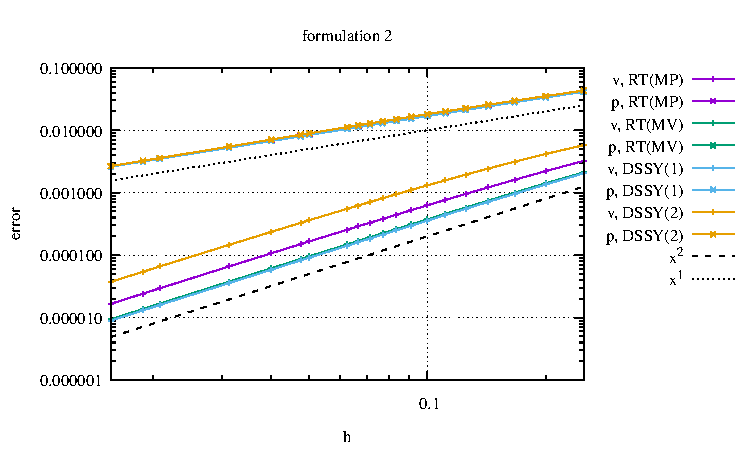
\includegraphics[width=8cm]{python_codes/fieldstone_77/results/dh/errors_form2}\\
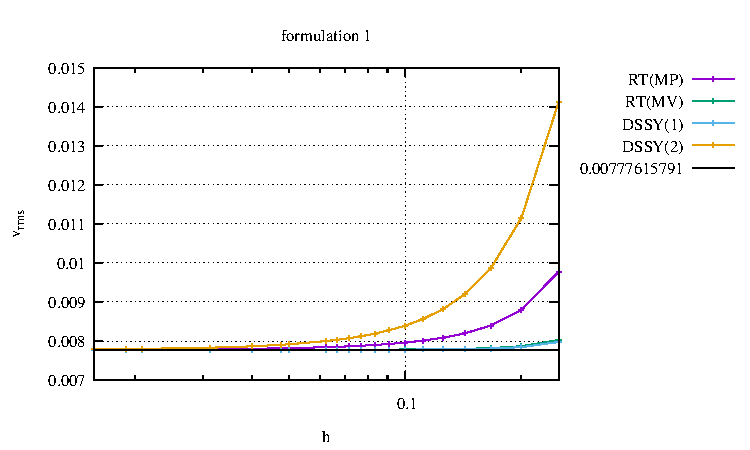
\includegraphics[width=8cm]{python_codes/fieldstone_77/results/dh/vrms_form1}
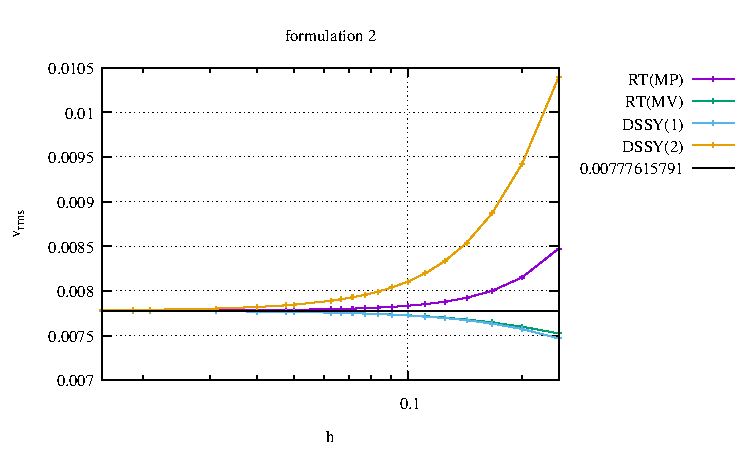
\includegraphics[width=8cm]{python_codes/fieldstone_77/results/dh/vrms_form2}\\
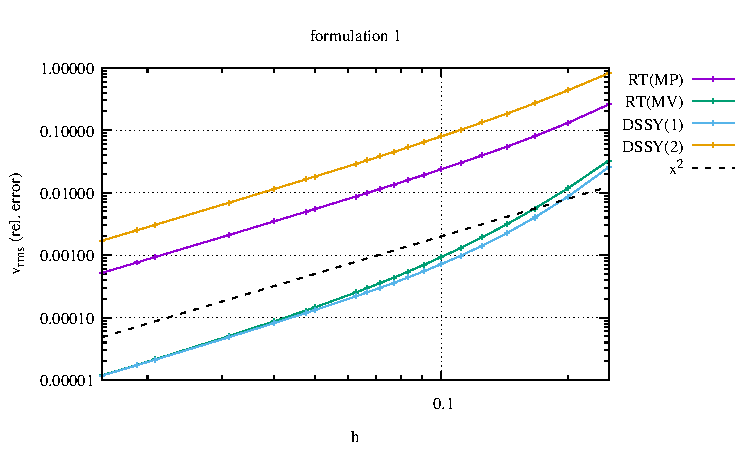
\includegraphics[width=8cm]{python_codes/fieldstone_77/results/dh/vrms_form1_relerror}
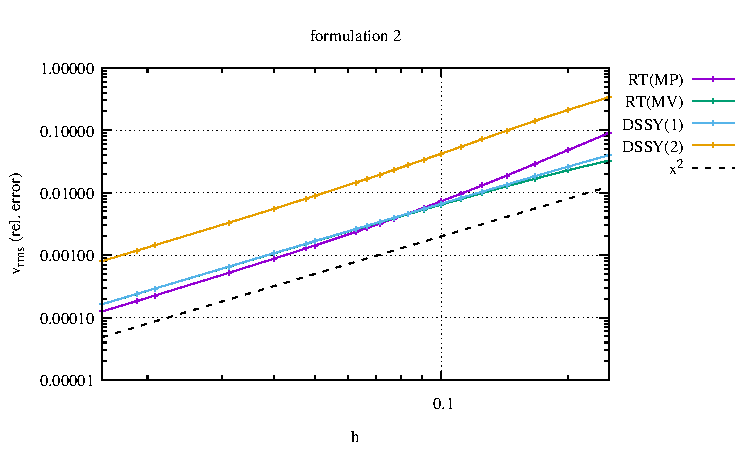
\includegraphics[width=8cm]{python_codes/fieldstone_77/results/dh/vrms_form2_relerror}\\
{\captionfont Top row: Velocity and pressure error convergence; 
Middle row: root mean square velocity. 
Bottom row: root mean square velocity relative error.}
\end{center}

\item Volker John benchmark \cite{jolm17}, see Section~\ref{ss:mms_jolm17}:

\begin{center}
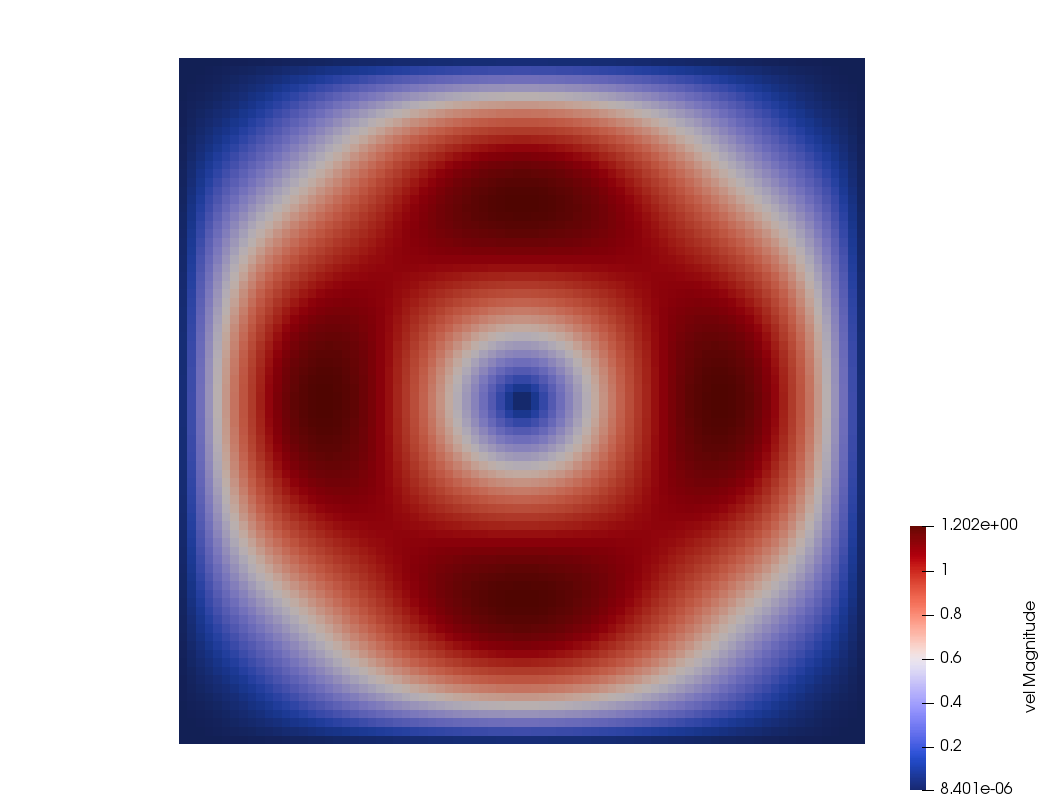
\includegraphics[width=7cm]{python_codes/fieldstone_77/results/vj/vel}
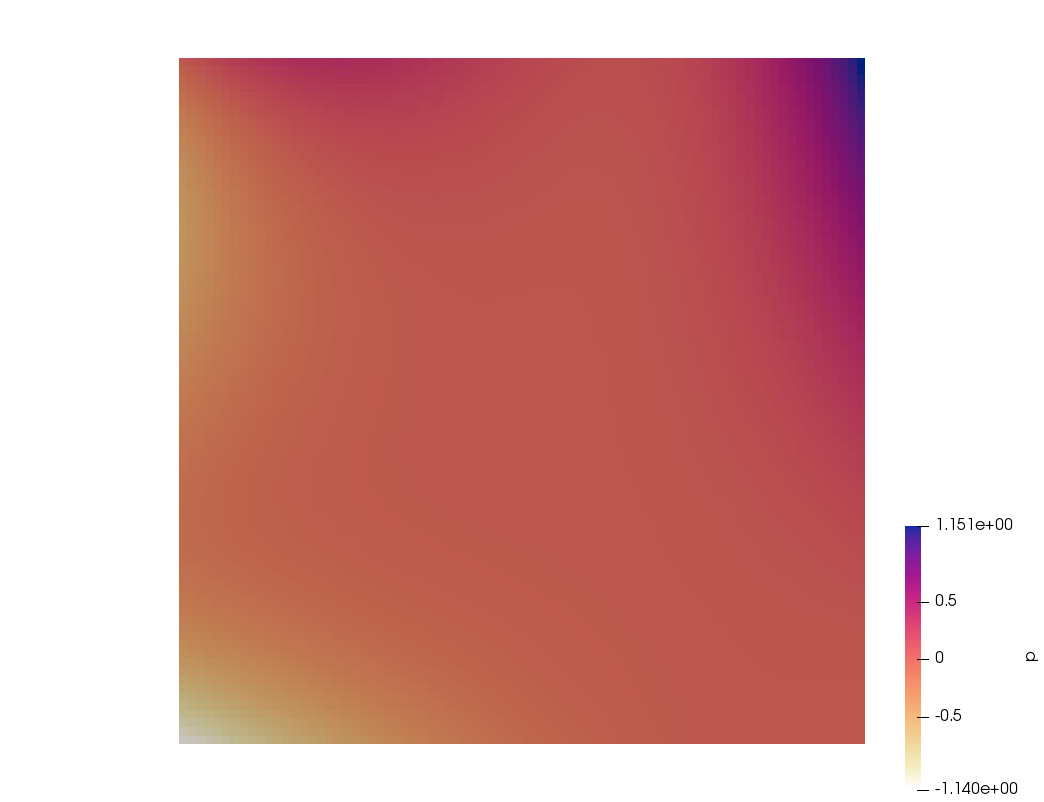
\includegraphics[width=7cm]{python_codes/fieldstone_77/results/vj/press}\\
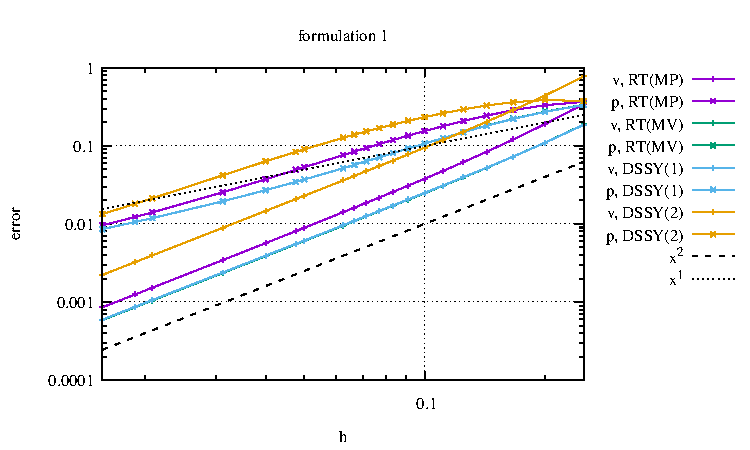
\includegraphics[width=8cm]{python_codes/fieldstone_77/results/vj/errors_form1}
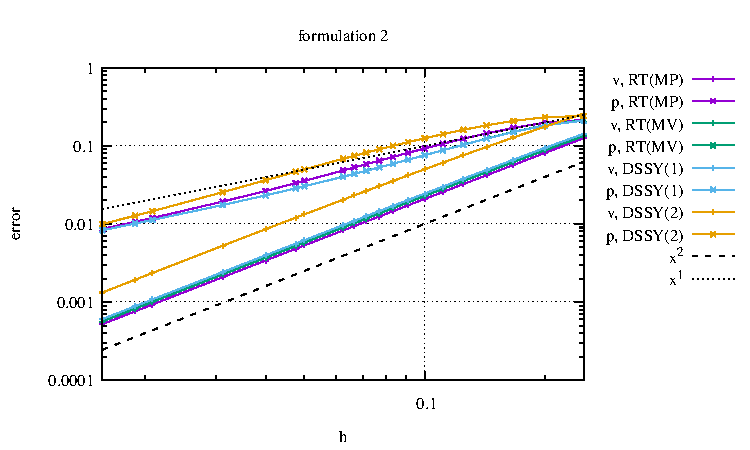
\includegraphics[width=8cm]{python_codes/fieldstone_77/results/vj/errors_form2}\\
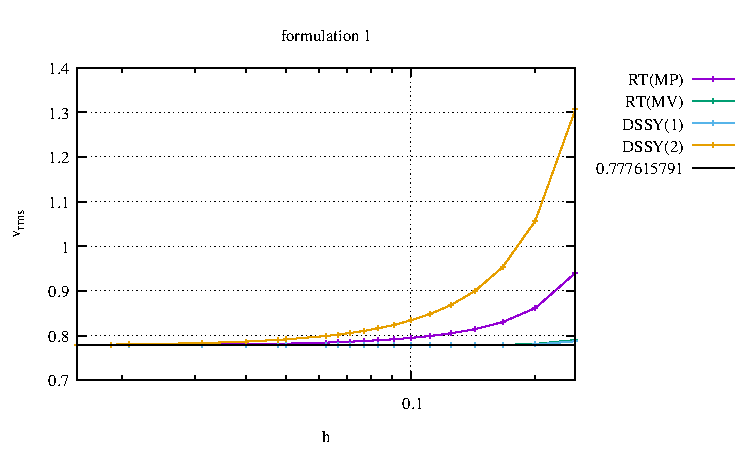
\includegraphics[width=8cm]{python_codes/fieldstone_77/results/vj/vrms_form1}
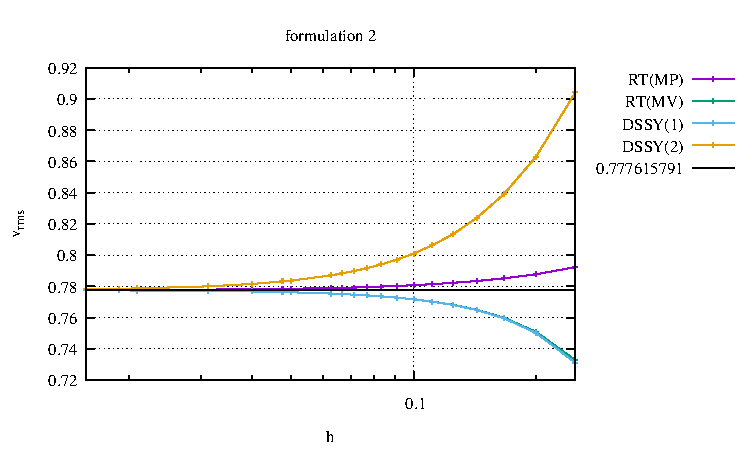
\includegraphics[width=8cm]{python_codes/fieldstone_77/results/vj/vrms_form2}\\
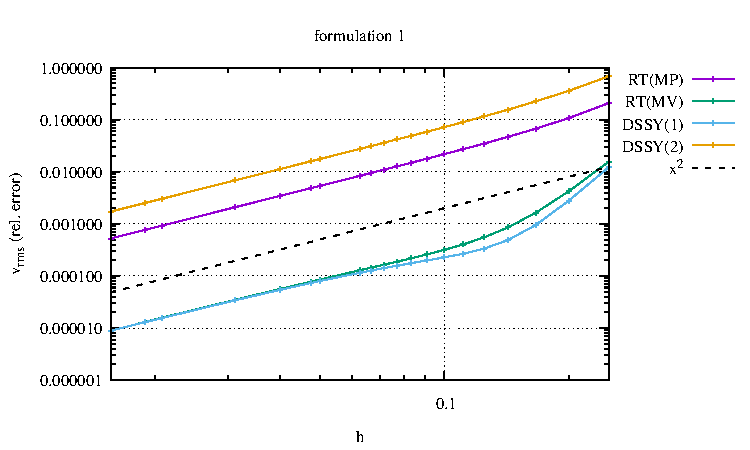
\includegraphics[width=8cm]{python_codes/fieldstone_77/results/vj/vrms_form1_relerror}
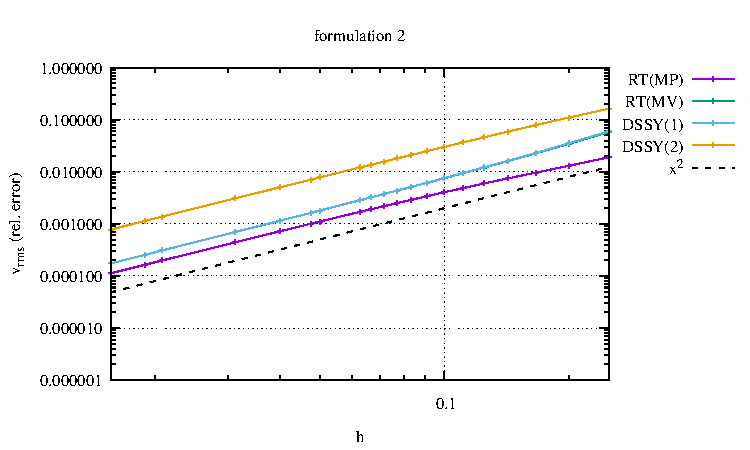
\includegraphics[width=8cm]{python_codes/fieldstone_77/results/vj/vrms_form2_relerror}\\
{\captionfont Top row: Velocity and pressure error convergence; 
Middle row: root mean square velocity. 
Bottom row: root mean square velocity relative error.}
\end{center}

\item Dohrmann \& Bochev 2D benchmark \cite{dobo04,bodg06}, see Section~\ref{ss:mms2}:

\begin{center}
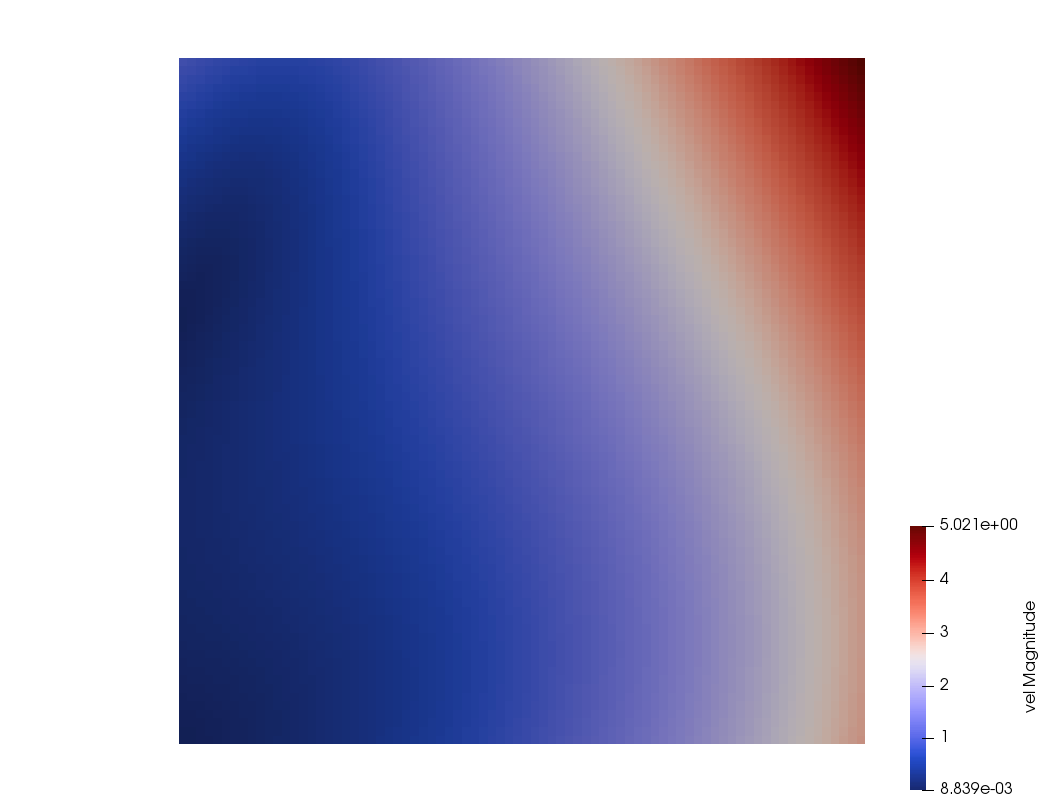
\includegraphics[width=7cm]{python_codes/fieldstone_77/results/db2D/vel}
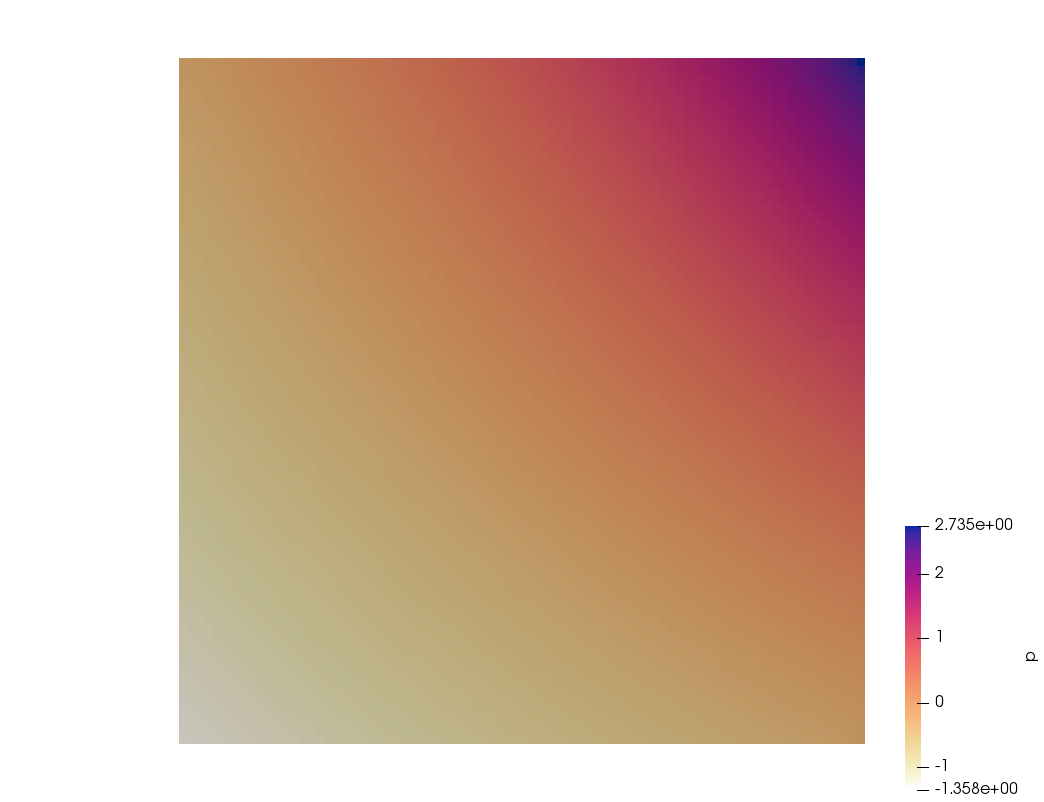
\includegraphics[width=7cm]{python_codes/fieldstone_77/results/db2D/press}\\
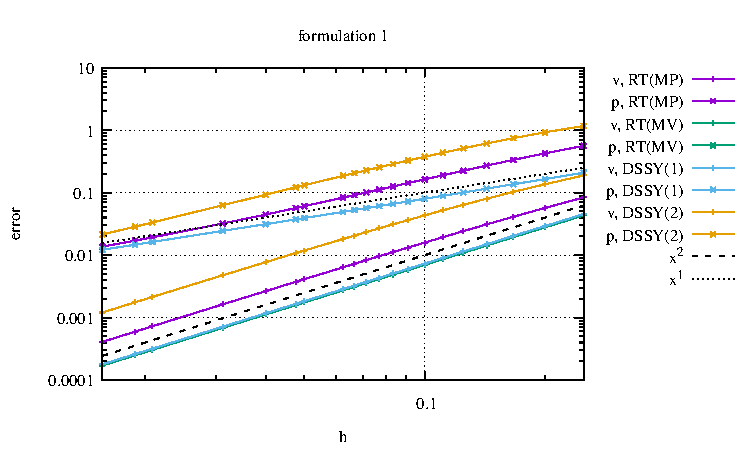
\includegraphics[width=8cm]{python_codes/fieldstone_77/results/db2D/errors_form1}
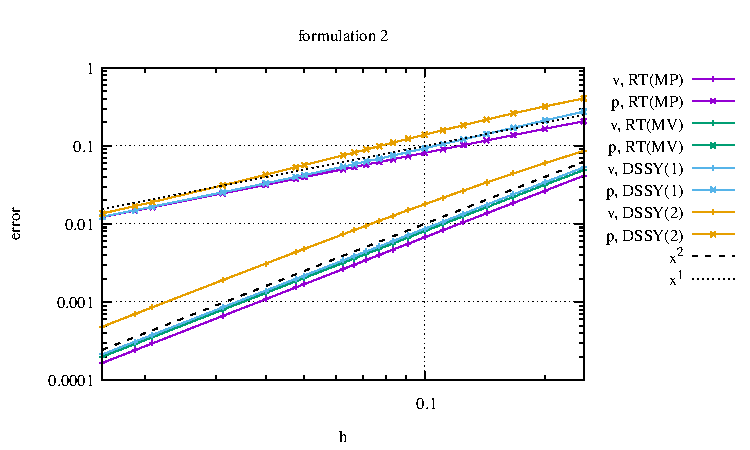
\includegraphics[width=8cm]{python_codes/fieldstone_77/results/db2D/errors_form2}\\
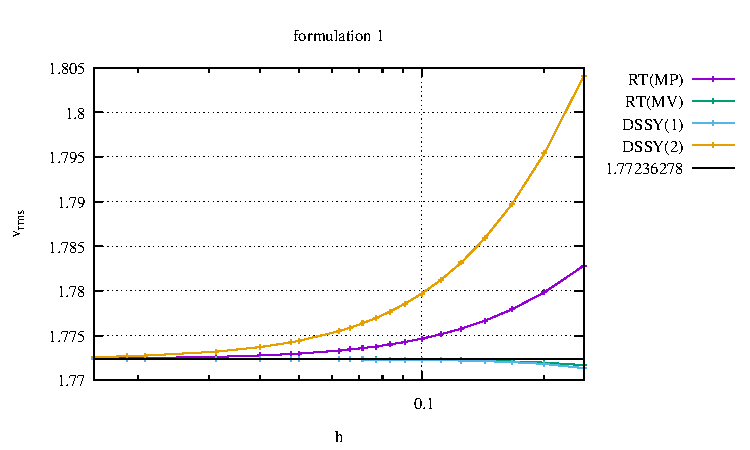
\includegraphics[width=8cm]{python_codes/fieldstone_77/results/db2D/vrms_form1}
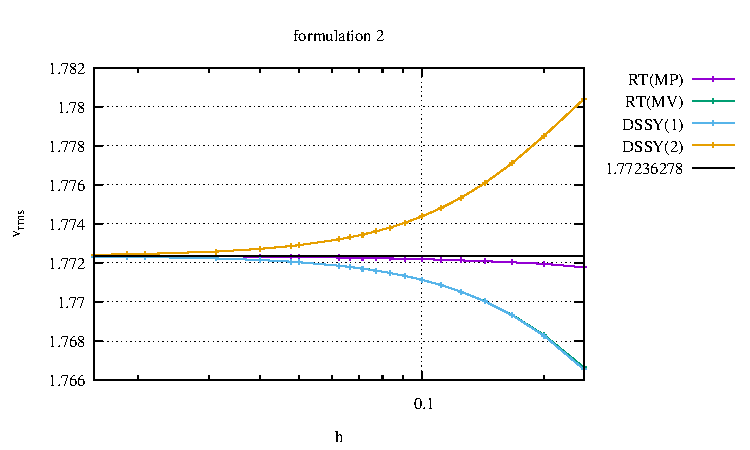
\includegraphics[width=8cm]{python_codes/fieldstone_77/results/db2D/vrms_form2}\\
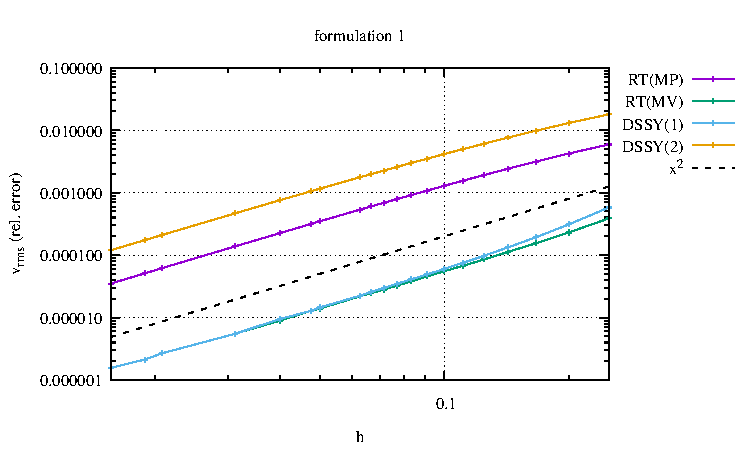
\includegraphics[width=8cm]{python_codes/fieldstone_77/results/db2D/vrms_form1_relerror}
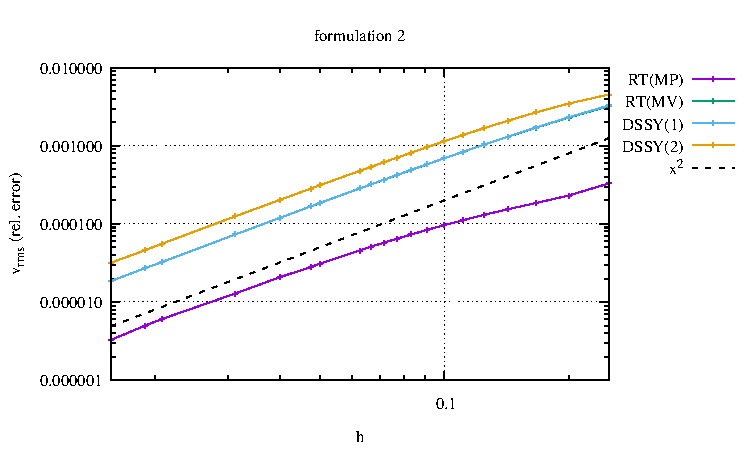
\includegraphics[width=8cm]{python_codes/fieldstone_77/results/db2D/vrms_form2_relerror}\\
{\captionfont Top row: Velocity and pressure error convergence; 
Middle row: root mean square velocity. 
Bottom row: root mean square velocity relative error.
Formulation 1 stands for the regular form of the 
Stokes equation, while formulation 2 stands for the Laplace one.}
\end{center}

\item SolCx benchmark, see \stone 5 (only formulation 1):

\begin{center}
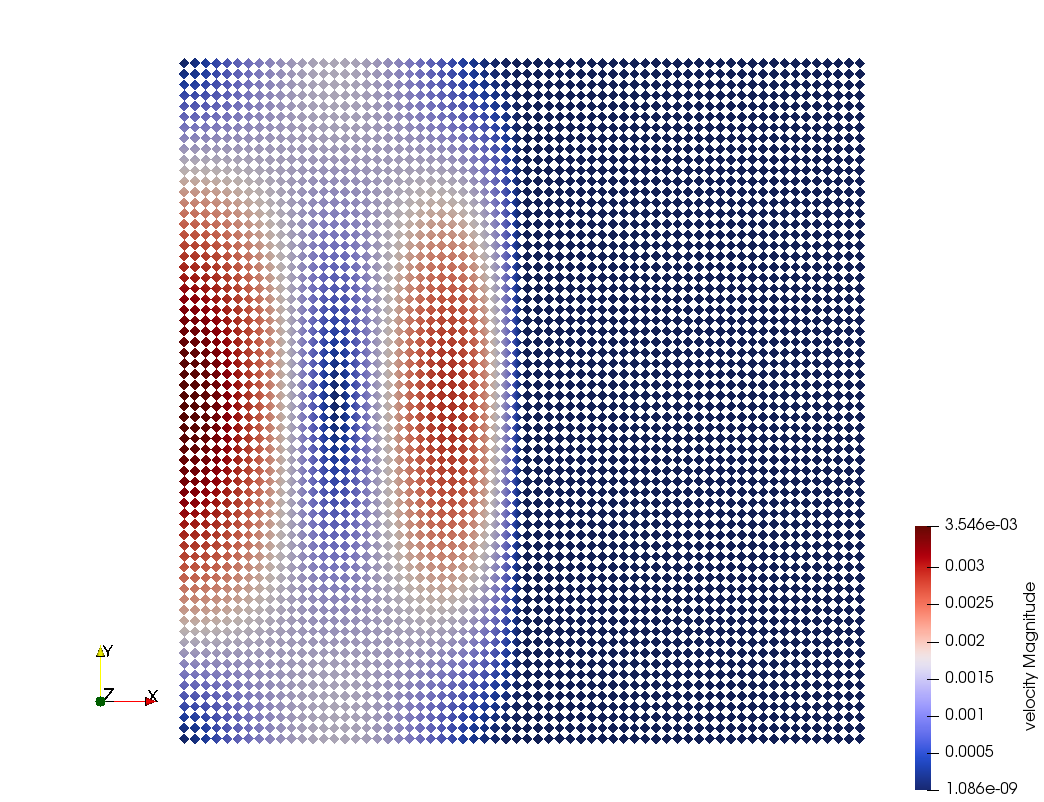
\includegraphics[width=7cm]{python_codes/fieldstone_77/results/solcx/vel}
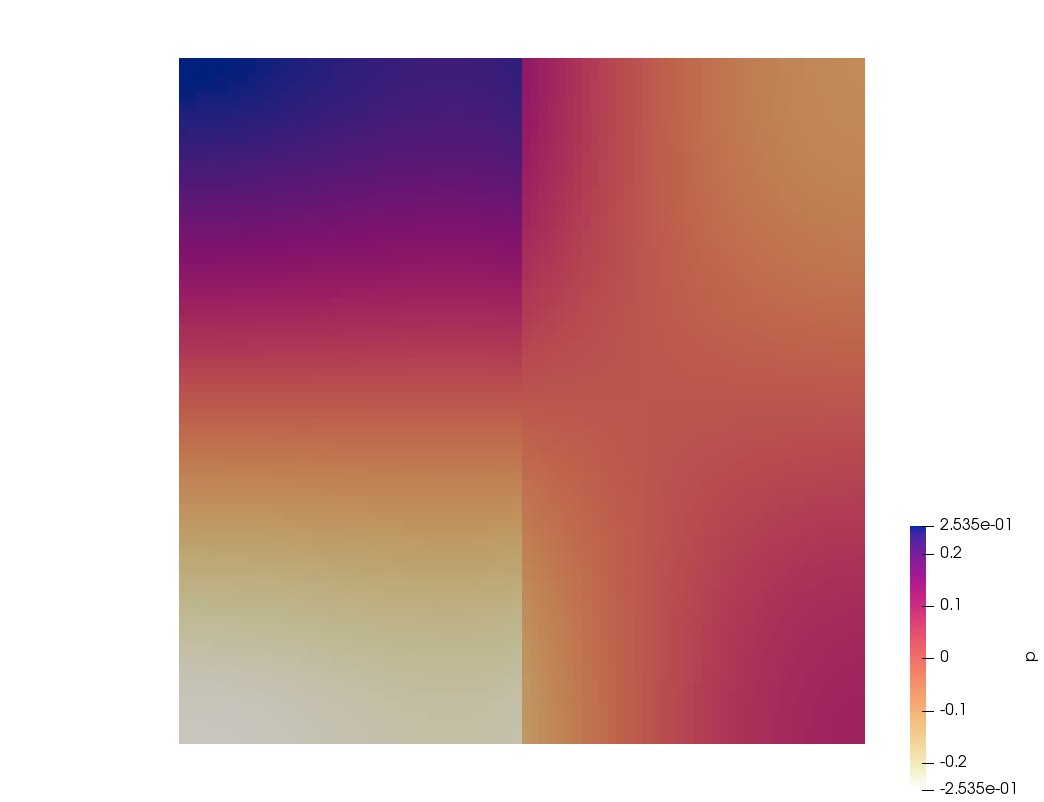
\includegraphics[width=7cm]{python_codes/fieldstone_77/results/solcx/press}\\
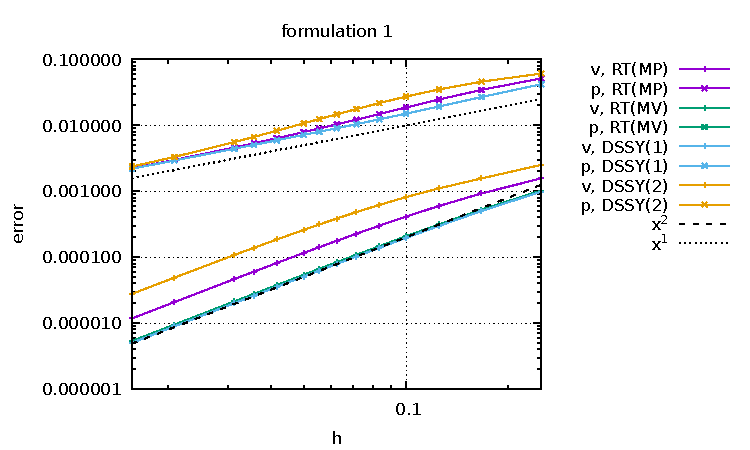
\includegraphics[width=8cm]{python_codes/fieldstone_77/results/solcx/errors_form1}
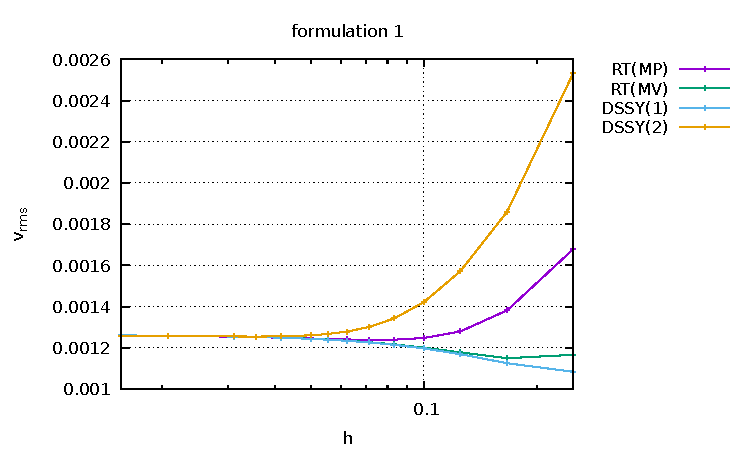
\includegraphics[width=8cm]{python_codes/fieldstone_77/results/solcx/vrms_form1}\\
{\captionfont Only even numbers of elements. Note that the paraview visualisation is based on 
quadrilaterals obtained by joining the nodes.}
\end{center}


\end{itemize}


Looking at these 4 analytical benchmarks (and focusing on the standard formulation only), 
we can conclude that RT(MV) and DSSY(1) are the two best elements and that they are very close to 
each other.



%........................................................................
\subsubsection*{Buoyancy-driven flow}

We see that both RT(MV) and DSSY(1) exhibit a quadratic convergence for the
velocity error and a linear convergence for the pressure error. Also the root mean square 
velocity measurements logically converge to their analytical values.  

Since these elements have been proven to be LBB stable one could think that it 
should then replace the standard $Q_1 \times P_0$: near identical cost, but LBB stable.

However, there is  a problem. I have also implemented another experiment: a unit cube domain
filled with a fluid of density $\rho_0=1$ and a cube of size $0.125\times 0.125$ centered in the domain
with density $\rho_0+\delta \rho$ with $\delta\rho=0.01$. The fluid has a viscosity $\eta=1$ while the 
block has a viscosity $\eta=1000$.
Boundary conditions are no slip on all sides, gravity points downwards with $|\vec{g}|=1$.

Results for all four basis functions are shown here:
\begin{center}
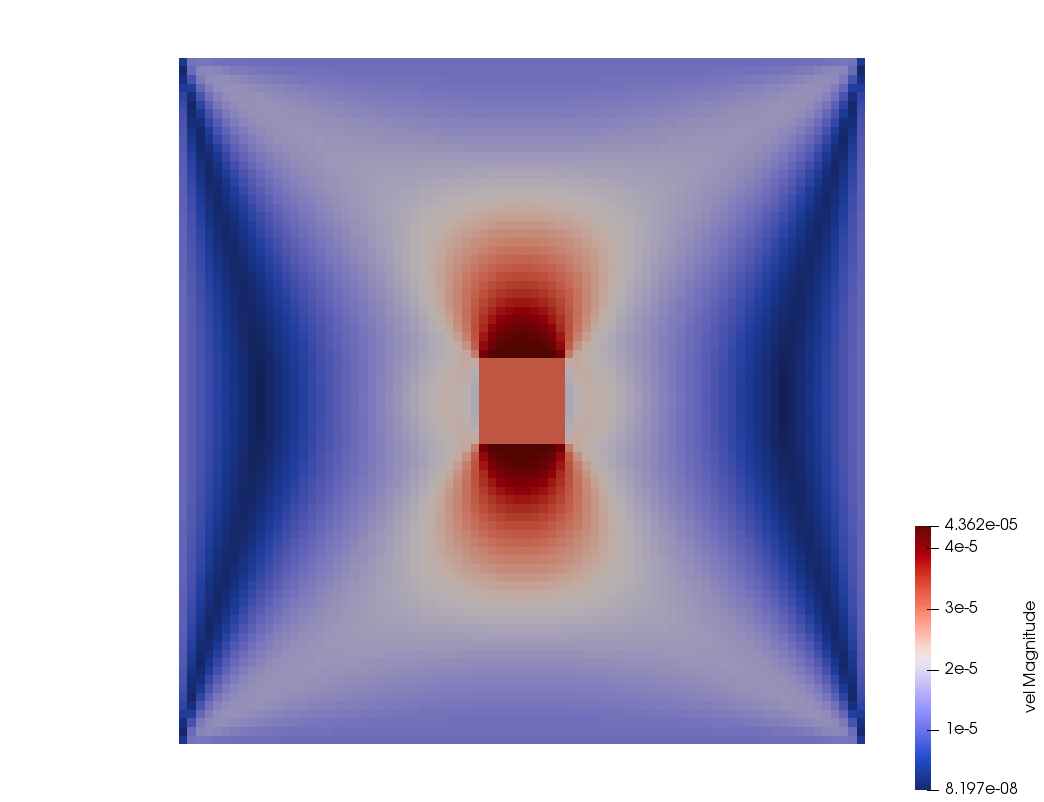
\includegraphics[width=4cm]{python_codes/fieldstone_77/results/block/full/vel1}
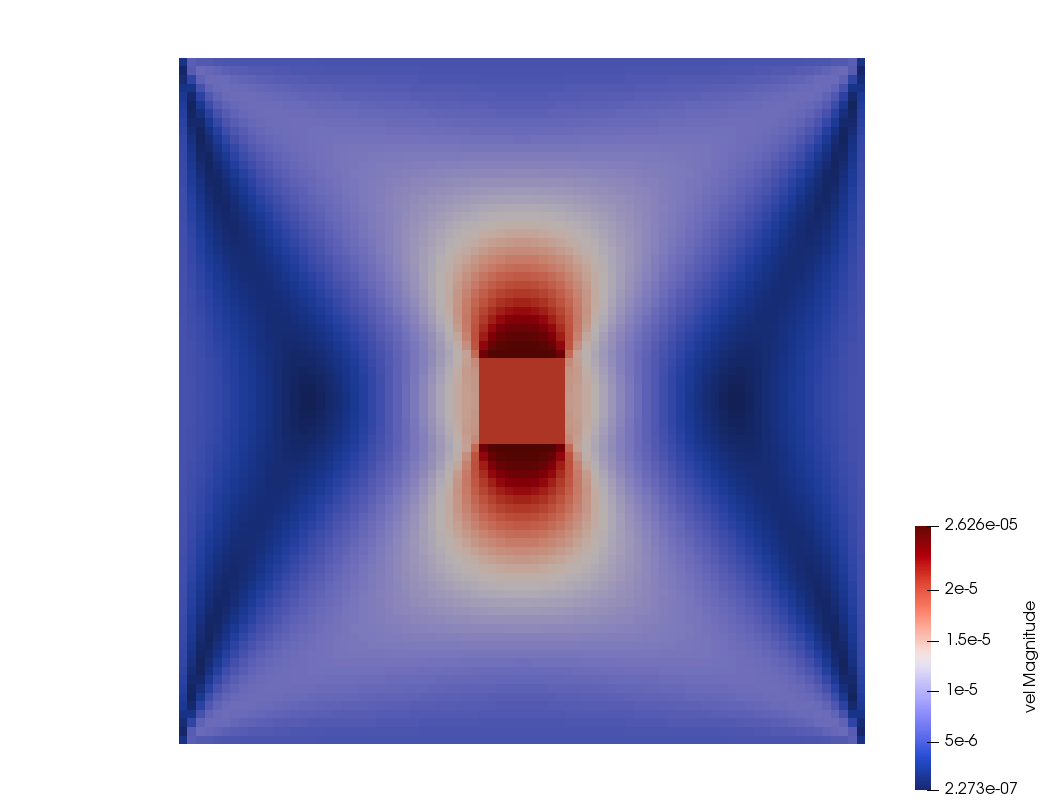
\includegraphics[width=4cm]{python_codes/fieldstone_77/results/block/full/vel2}
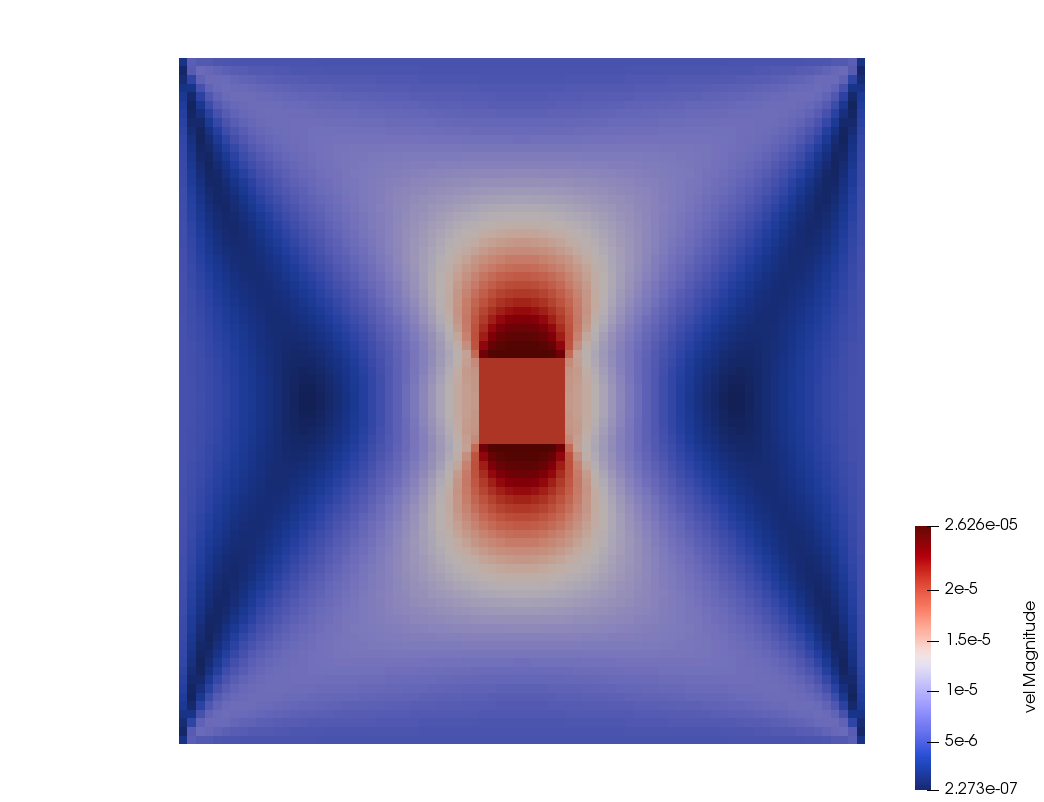
\includegraphics[width=4cm]{python_codes/fieldstone_77/results/block/full/vel3}
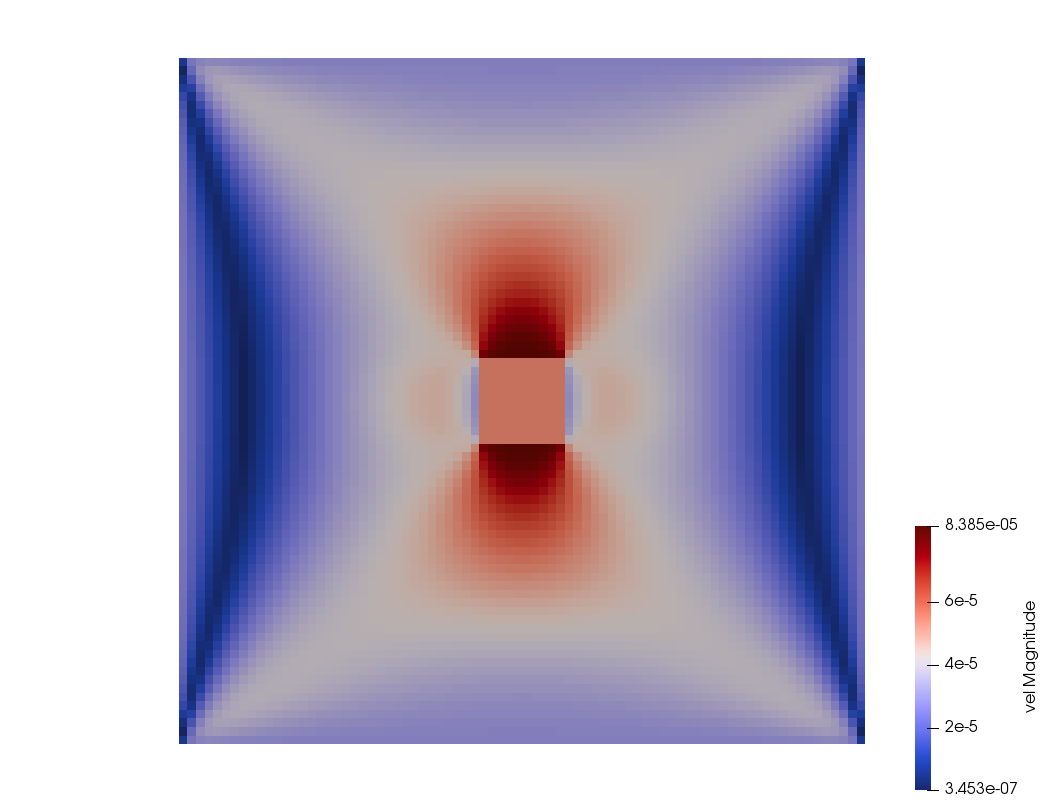
\includegraphics[width=4cm]{python_codes/fieldstone_77/results/block/full/vel4}\\
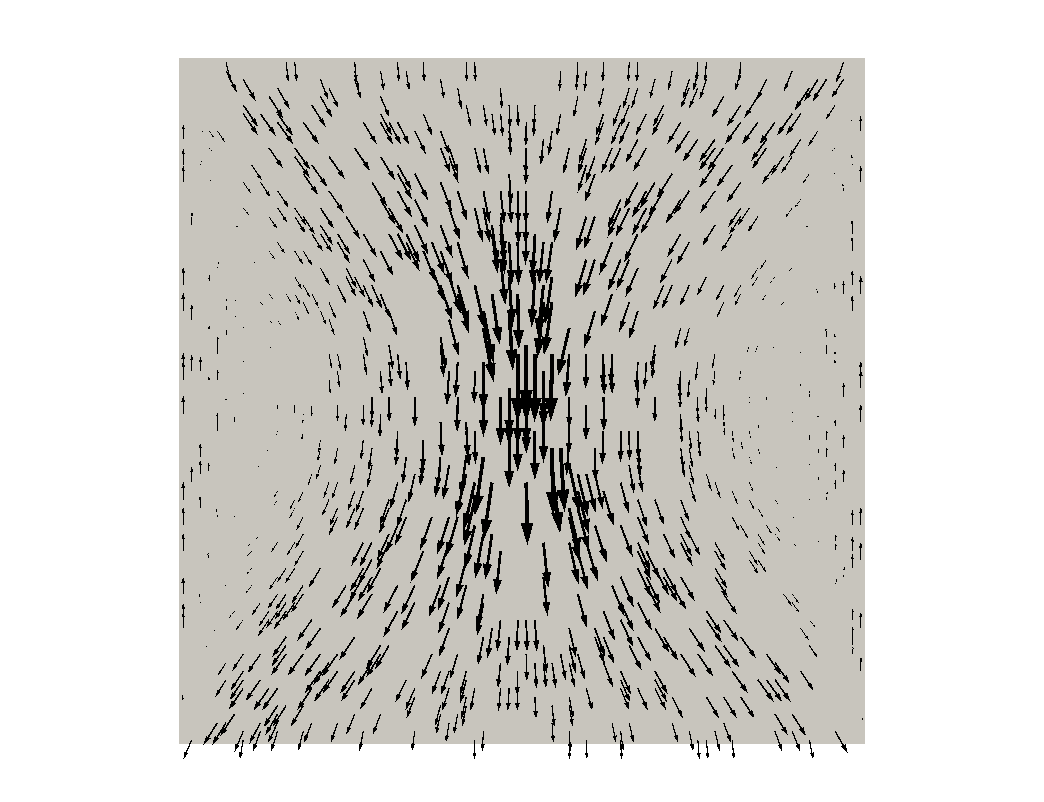
\includegraphics[width=4cm]{python_codes/fieldstone_77/results/block/full/vels1}
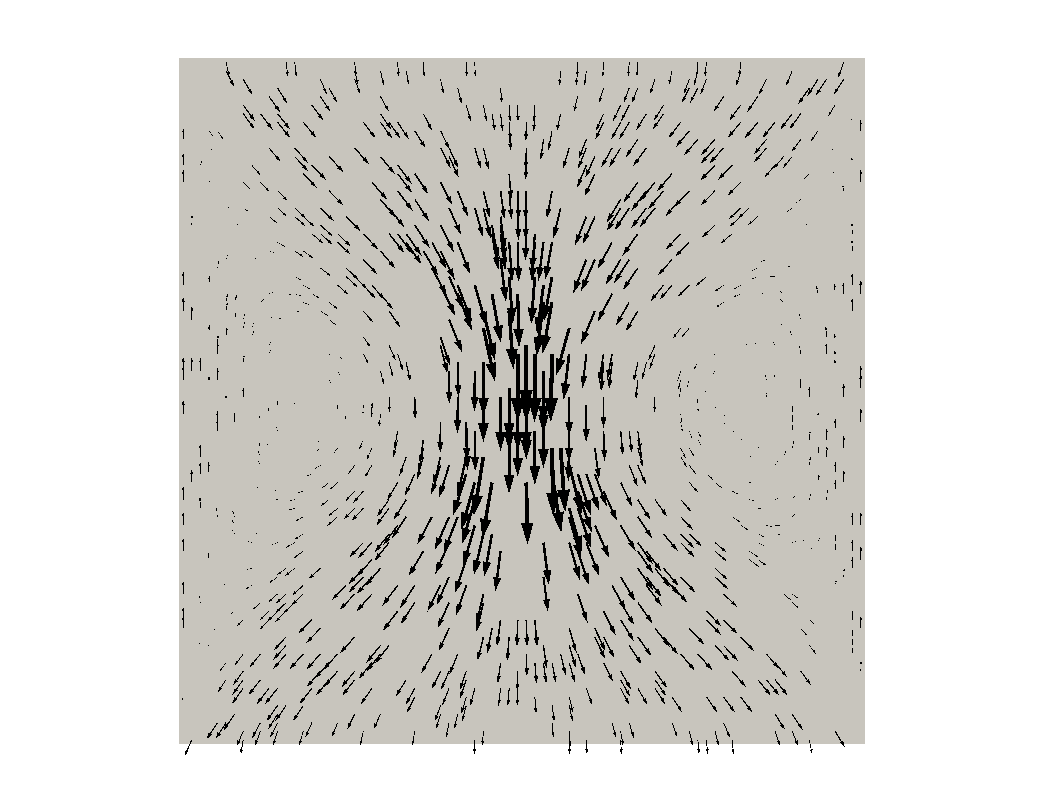
\includegraphics[width=4cm]{python_codes/fieldstone_77/results/block/full/vels2}
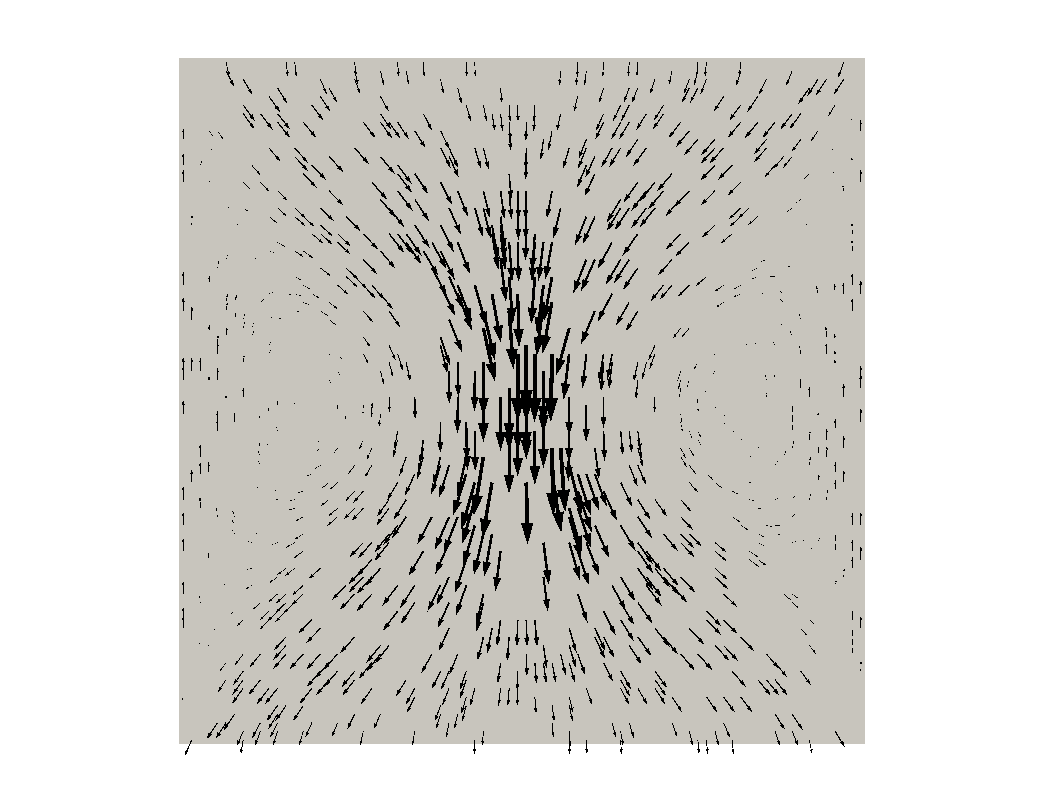
\includegraphics[width=4cm]{python_codes/fieldstone_77/results/block/full/vels3}
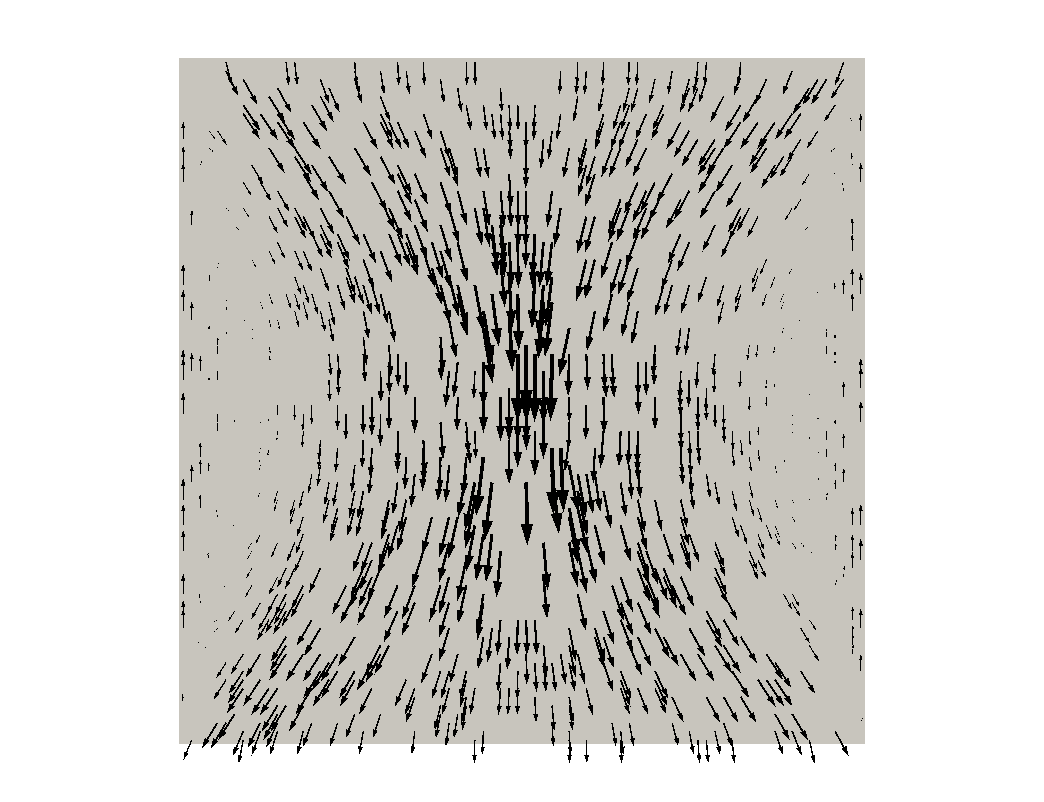
\includegraphics[width=4cm]{python_codes/fieldstone_77/results/block/full/vels4}\\
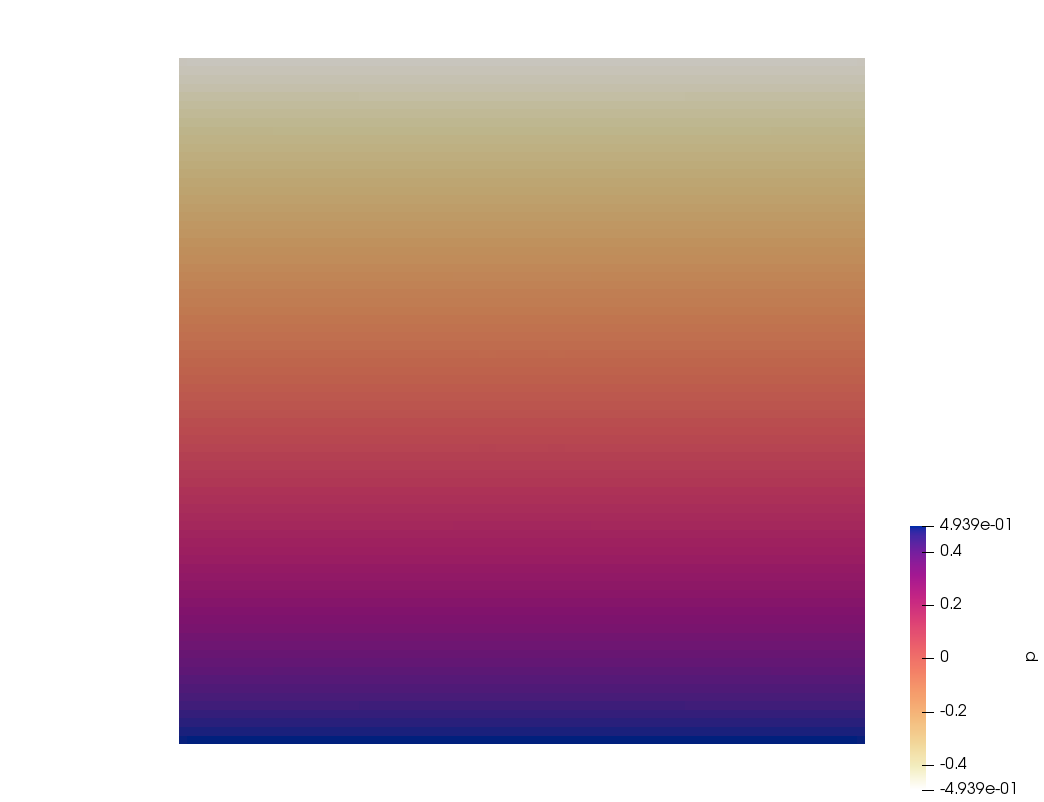
\includegraphics[width=4cm]{python_codes/fieldstone_77/results/block/full/press1}
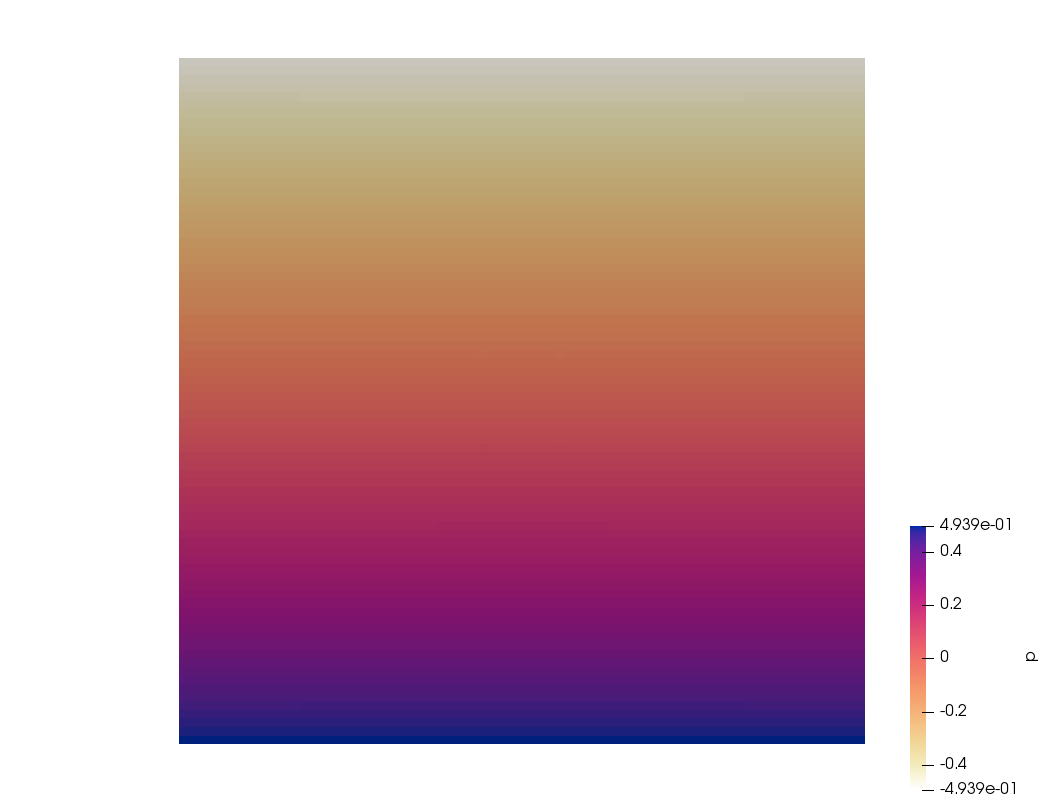
\includegraphics[width=4cm]{python_codes/fieldstone_77/results/block/full/press2}
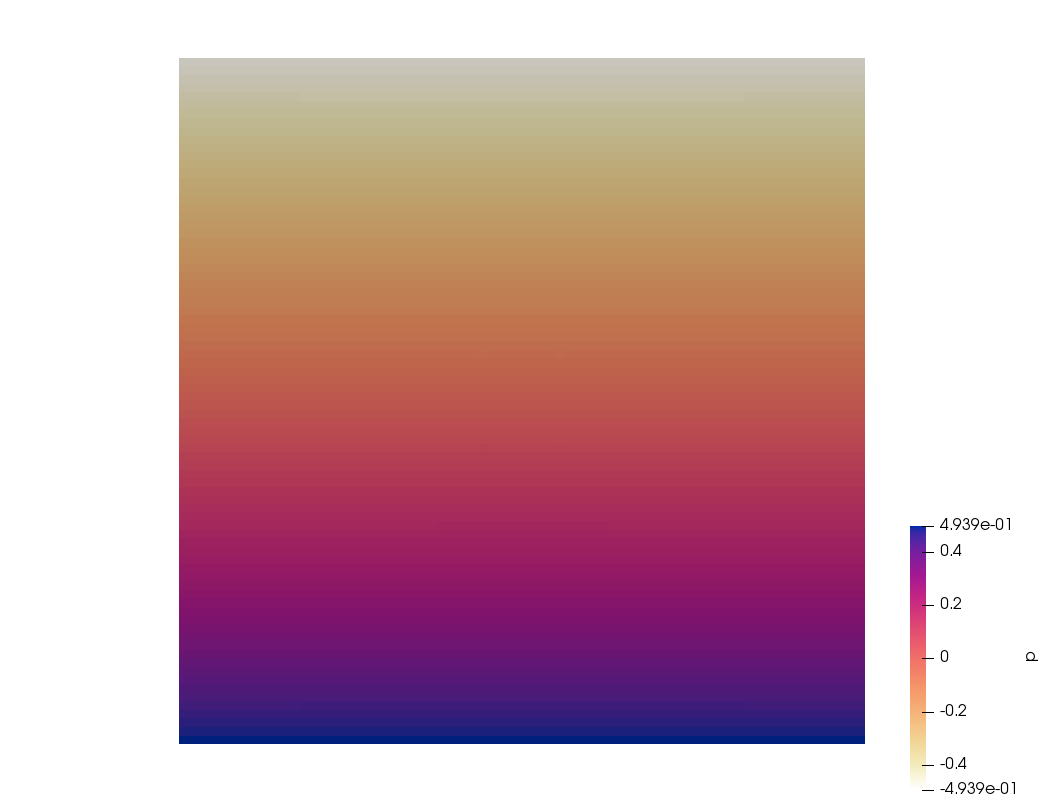
\includegraphics[width=4cm]{python_codes/fieldstone_77/results/block/full/press3}
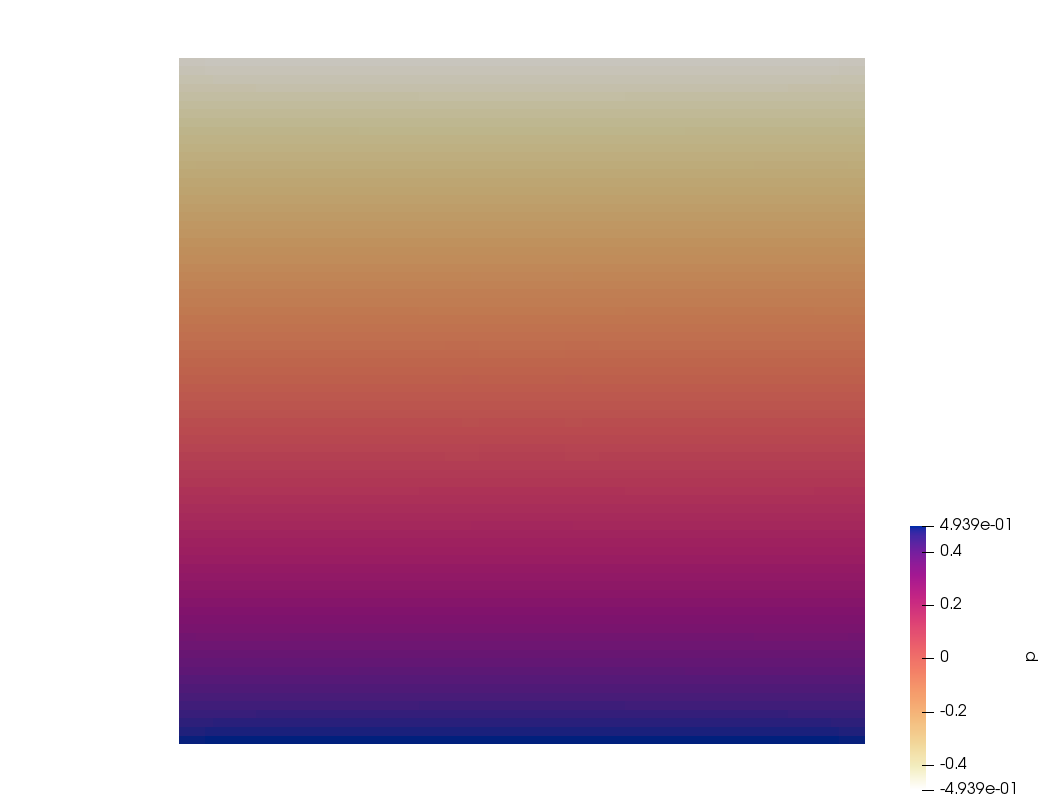
\includegraphics[width=4cm]{python_codes/fieldstone_77/results/block/full/press4}\\
{\captionfont Full density. Left to right: RT(MP), RT(MV), DSSY(1), DSSY(2). 64x64 elements}
\end{center}

We see that the pressure field is lithostatic and chequerboard-free  but the velocity field is abnormal 
(we expect a convection cell on each side of the cube).
If I now re-run these experiments in reduced density ($\rho_0=0$) then we recover
the expected velocity field\footnote{Not saying it is 'the' solution but it at least makes sense}:

\begin{center}
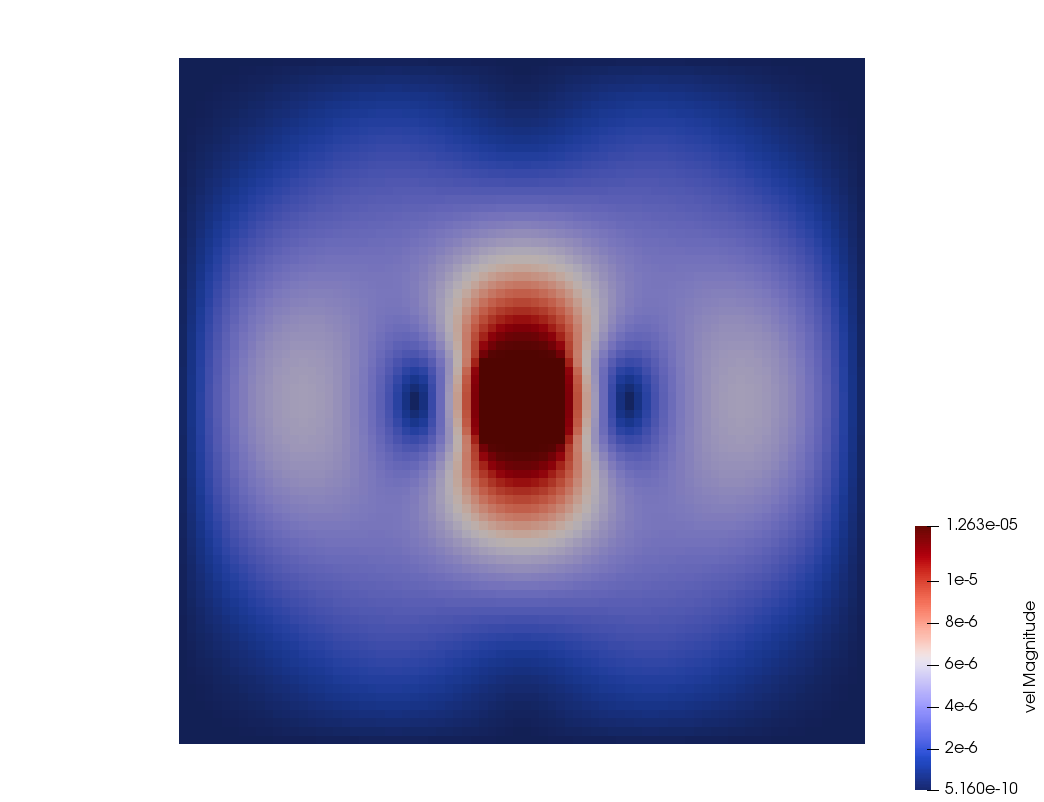
\includegraphics[width=4cm]{python_codes/fieldstone_77/results/block/reduced/vel1}
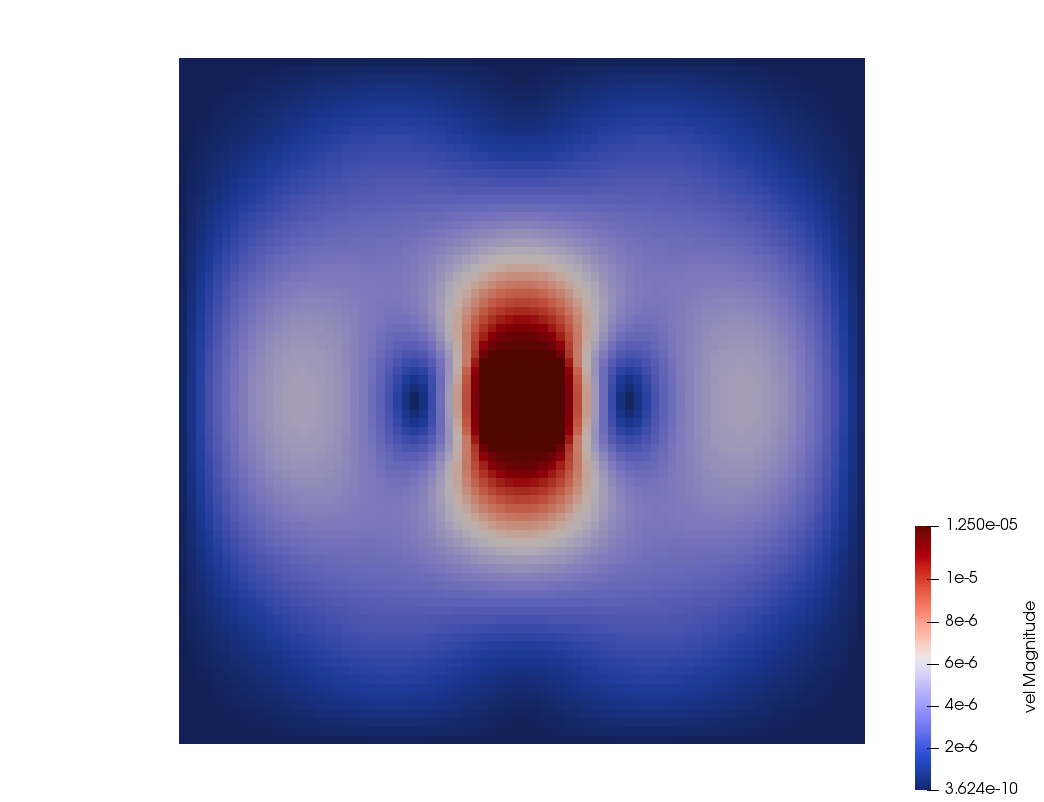
\includegraphics[width=4cm]{python_codes/fieldstone_77/results/block/reduced/vel2}
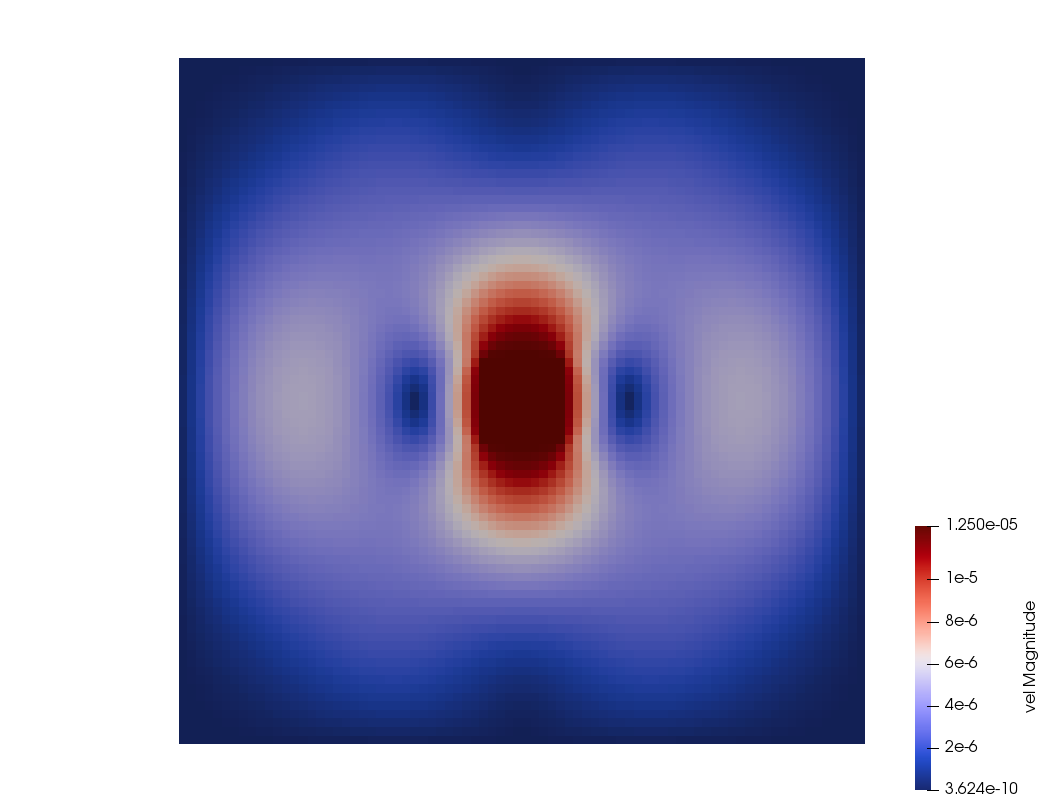
\includegraphics[width=4cm]{python_codes/fieldstone_77/results/block/reduced/vel3}
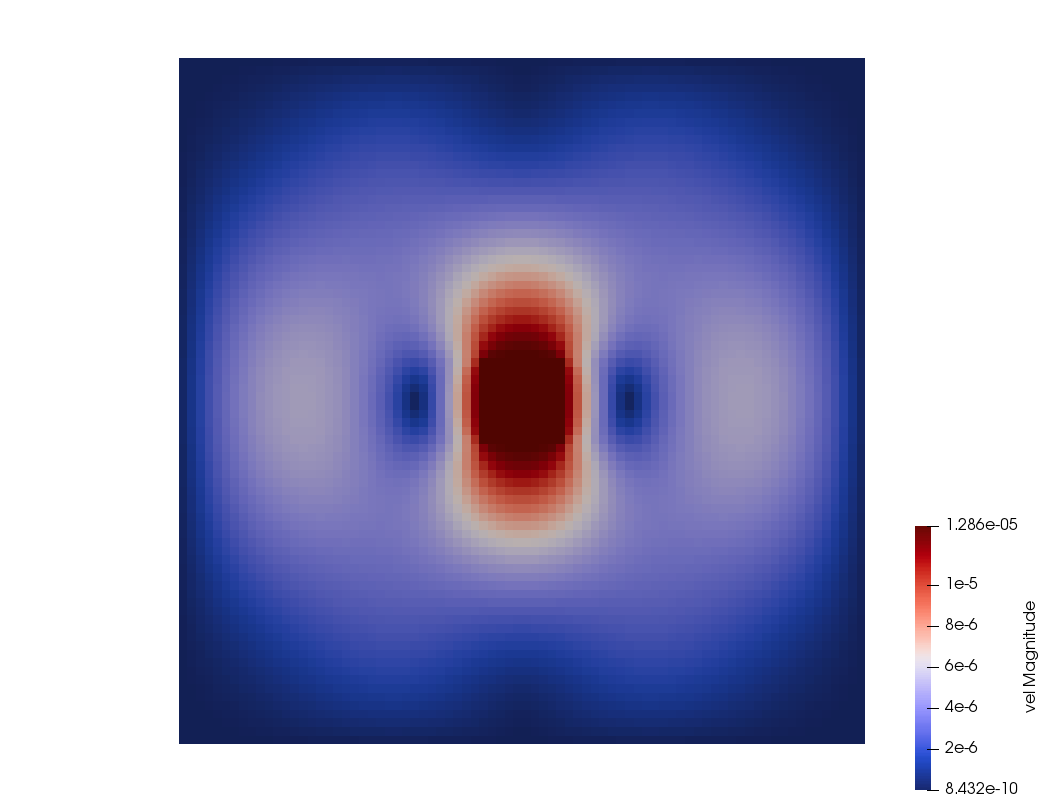
\includegraphics[width=4cm]{python_codes/fieldstone_77/results/block/reduced/vel4}\\
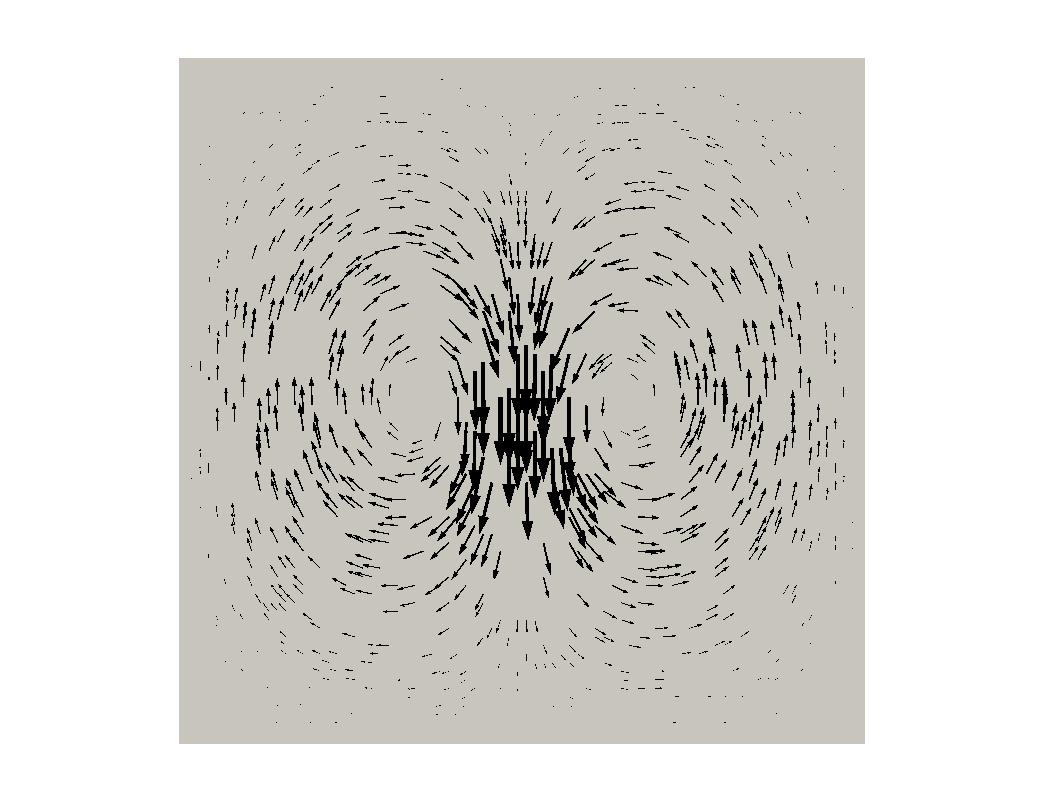
\includegraphics[width=4cm]{python_codes/fieldstone_77/results/block/reduced/vels1}
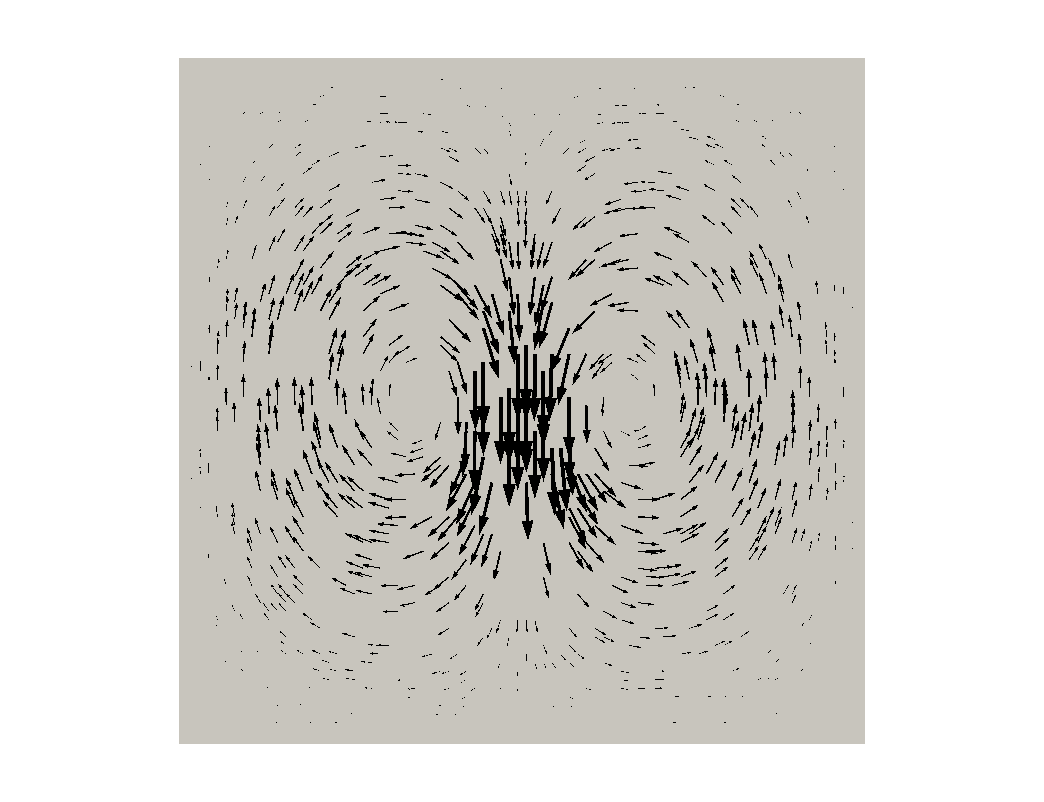
\includegraphics[width=4cm]{python_codes/fieldstone_77/results/block/reduced/vels2}
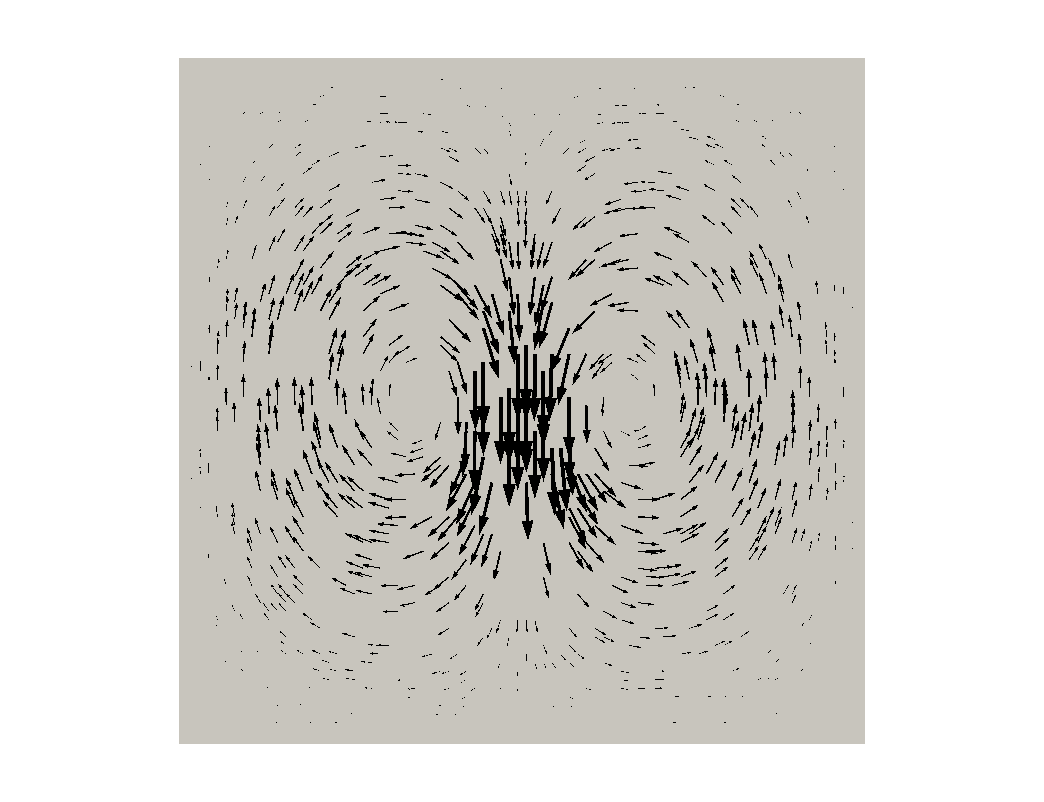
\includegraphics[width=4cm]{python_codes/fieldstone_77/results/block/reduced/vels3}
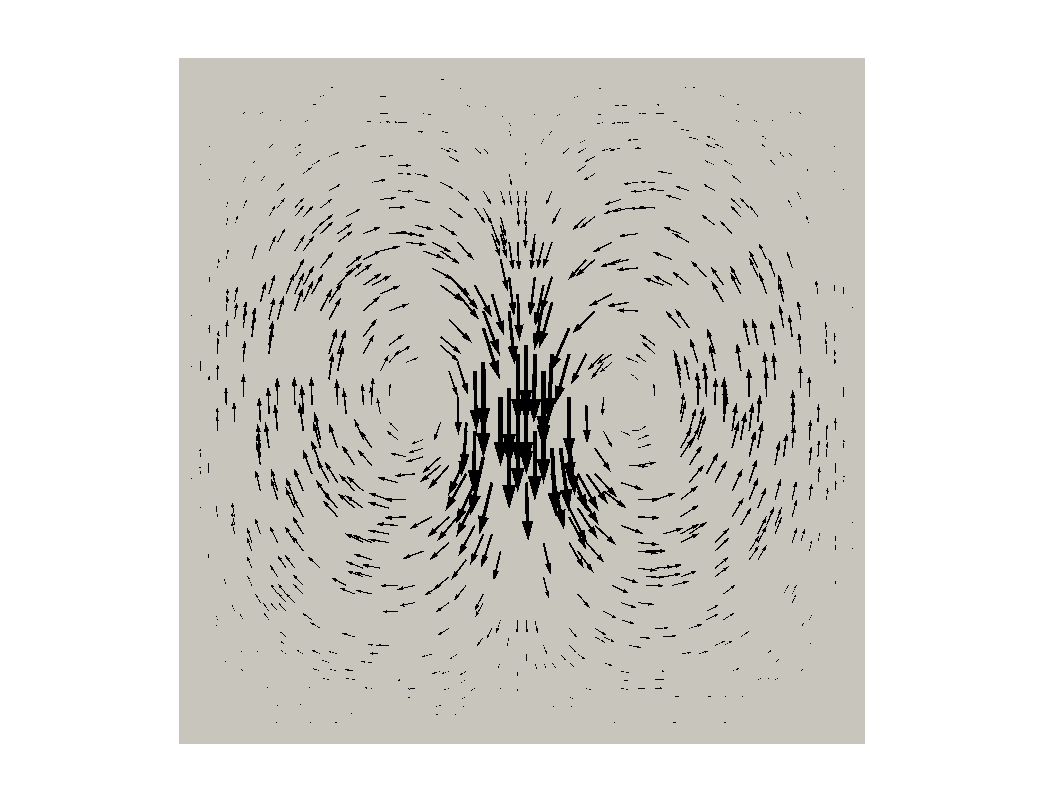
\includegraphics[width=4cm]{python_codes/fieldstone_77/results/block/reduced/vels4}\\
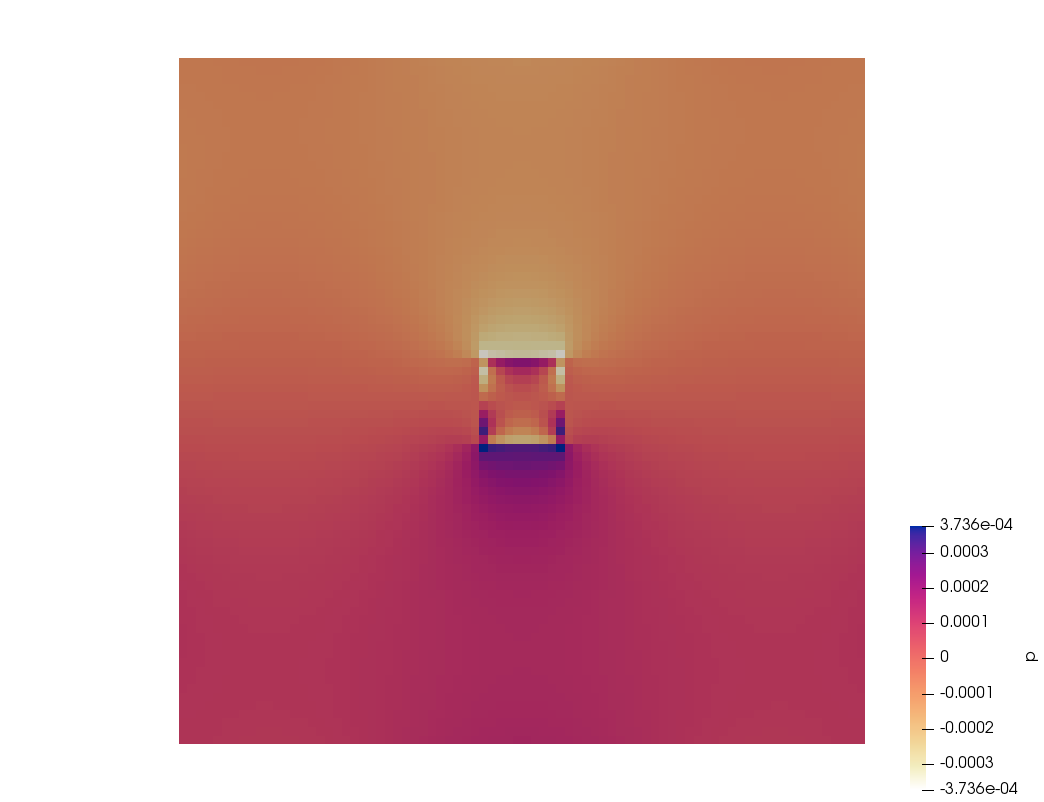
\includegraphics[width=4cm]{python_codes/fieldstone_77/results/block/reduced/press1}
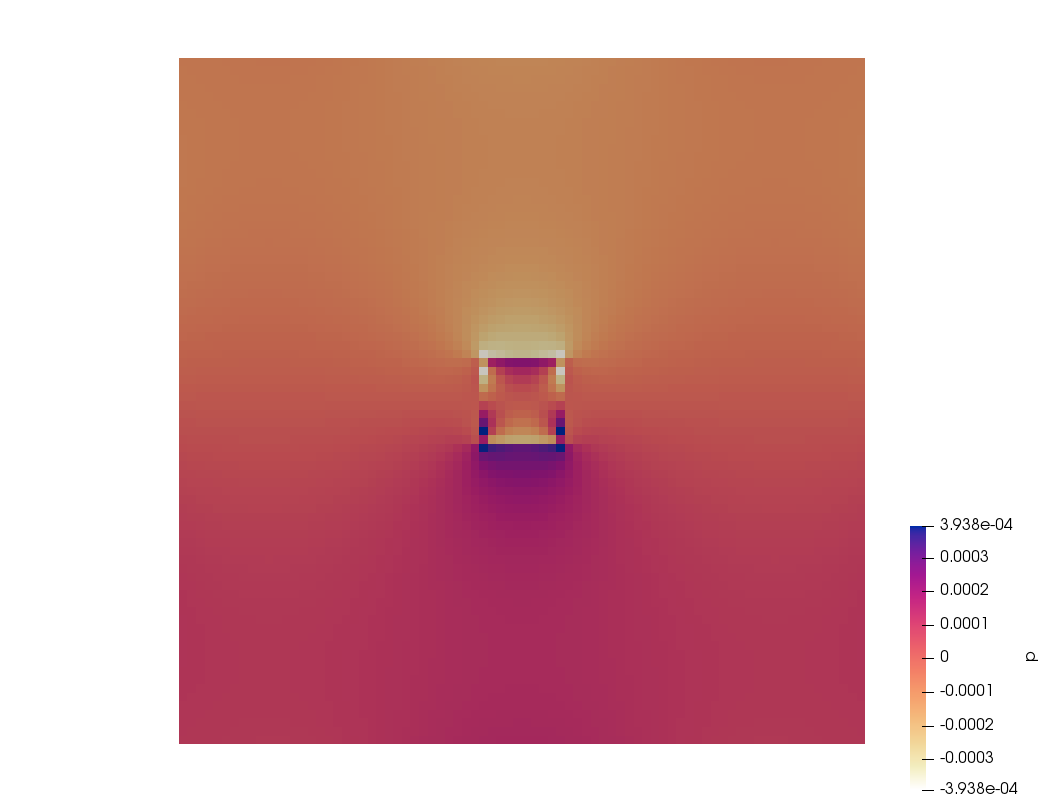
\includegraphics[width=4cm]{python_codes/fieldstone_77/results/block/reduced/press2}
\includegraphics[width=4cm]{python_codes/fieldstone_77/results/block/reduced/press3}
\includegraphics[width=4cm]{python_codes/fieldstone_77/results/block/reduced/press4}\\
{\captionfont Reduced density. Left to right: RT(MP), RT(MV), DSSY(1), DSSY(2). 64x64 elements}
\end{center}


If I now conduct a short study on the value of $\delta\rho$:

\begin{center}
\includegraphics[width=5cm]{python_codes/fieldstone_77/results/block/drho/vel1}
\includegraphics[width=5cm]{python_codes/fieldstone_77/results/block/drho/vel3}
\includegraphics[width=5cm]{python_codes/fieldstone_77/results/block/drho/vel2}\\
\includegraphics[width=5cm]{python_codes/fieldstone_77/results/block/drho/vels1}
\includegraphics[width=5cm]{python_codes/fieldstone_77/results/block/drho/vels3}
\includegraphics[width=5cm]{python_codes/fieldstone_77/results/block/drho/vels2}\\
\includegraphics[width=5cm]{python_codes/fieldstone_77/results/block/drho/press1}
\includegraphics[width=5cm]{python_codes/fieldstone_77/results/block/drho/press3}
\includegraphics[width=5cm]{python_codes/fieldstone_77/results/block/drho/press2}\\
{\captionfont From left to right: $\delta \rho=1,0.1,0.01$. 80x80 elements.}
\end{center}

The conclusion is clear: in its current form, and unless there is a fundamental 
flaw in my implementation\footnote{but then how could the anlalytical benchmarks work 
so well?}, these elements are not capable to 
deal with buoyancy-driven flows where $\delta \rho/\rho < 1-10\%$ which is 
unfortunately the type of simulations that are carried out in mantle dynamics modelling.
The reasons are (partially) discussed in Section~\ref{ss:RTq1p0}, but 
I am not sure how to go further. If an additional jump term is needed in the 
weak form in order to fix this problem, this makes the element not as simple as
advertised. 





